\documentclass{beamer}

\usepackage{graphicx}
\usepackage{fontspec}
\usepackage[scale=0.9,sfdefault,light]{roboto}
\usepackage{listings}

\definecolor{unusedline}{gray}{0.7}

\graphicspath{ {img/} }

\usetheme{Marburg}
\usecolortheme{whale}

\title{git essential}
\subtitle{git essential}
\date{\today}

\begin{document}

\begin{frame}
    \begin{figure}
        \center
        
\includegraphics{git-logo}
        \label{fig:git-logo}
    \end{figure}
    \center{git essential}
    \center{ \tiny{Sitdhibong Laokok} }
\end{frame}

\begin{frame}
    \begin{figure}
        \center
        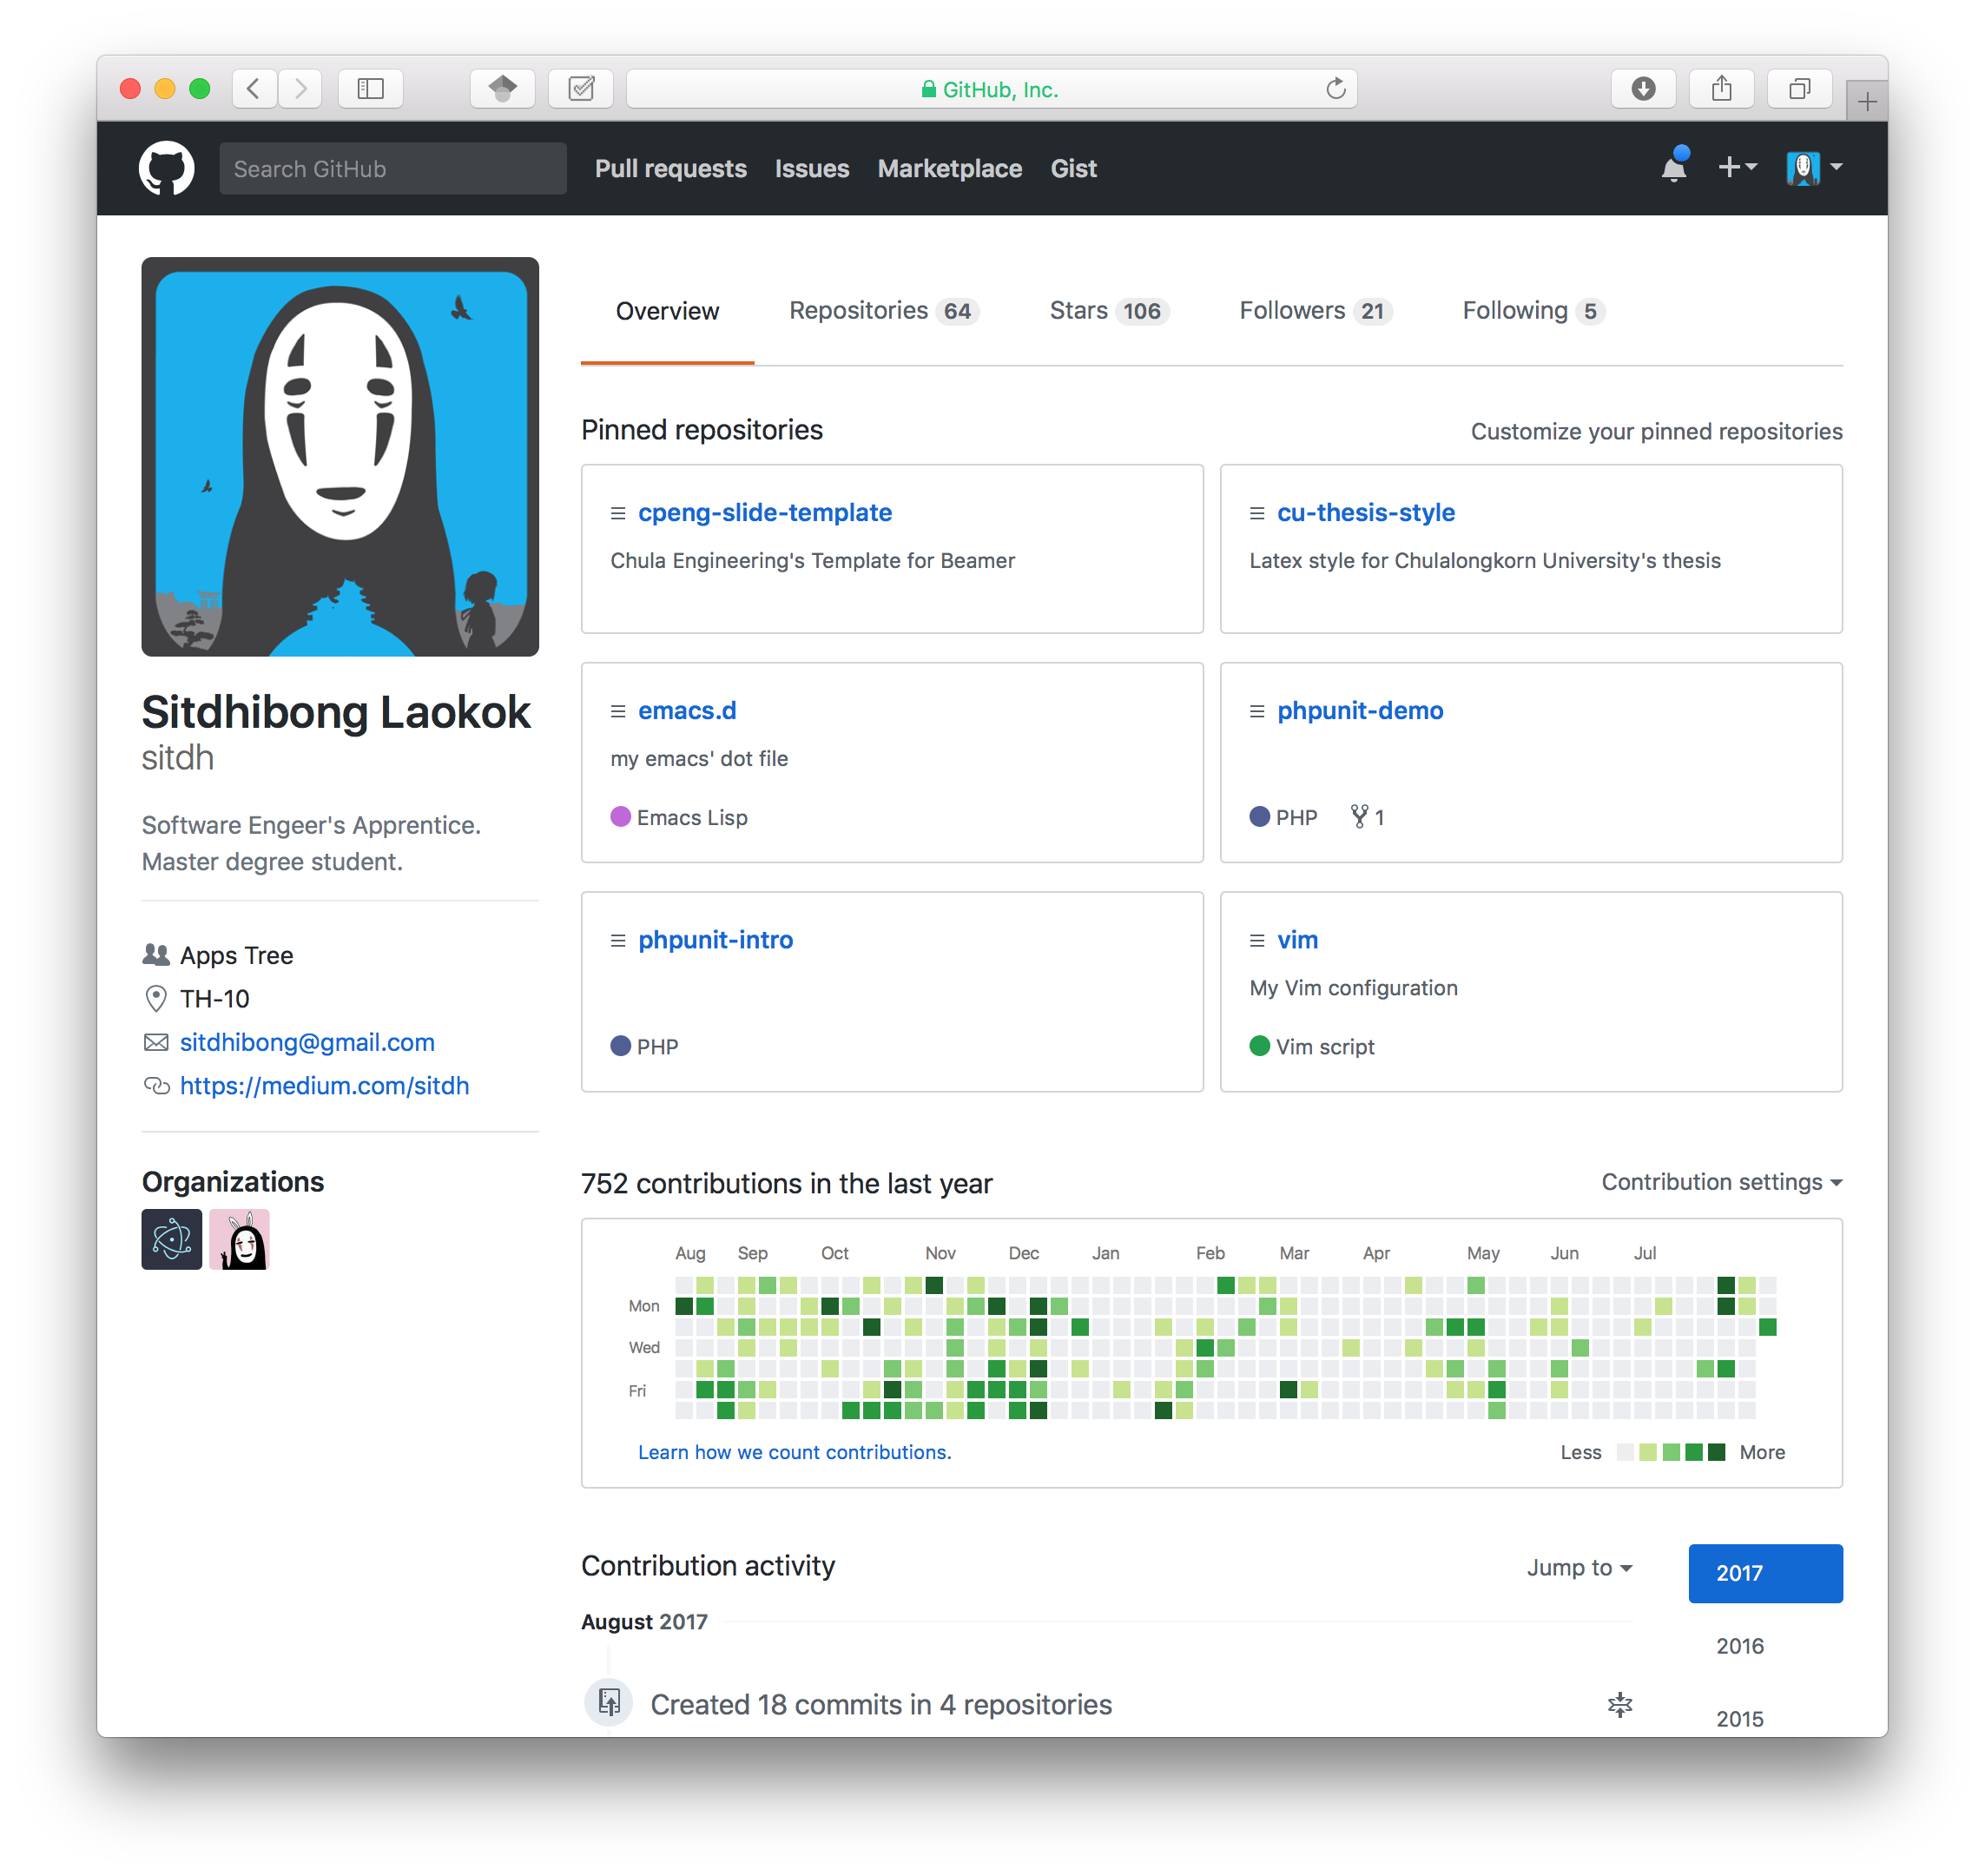
\includegraphics[width=.8\textwidth]{git-profile}
        \caption{https://github.com/sitdh}
        \label{fig:git-profile}
    \end{figure}
\end{frame}

\begin{frame}
    \frametitle{Outline}
    \tableofcontents
\end{frame}

\section{Activity flow}
\begin{frame}{Activity flow}
    \begin{figure}
        \center
        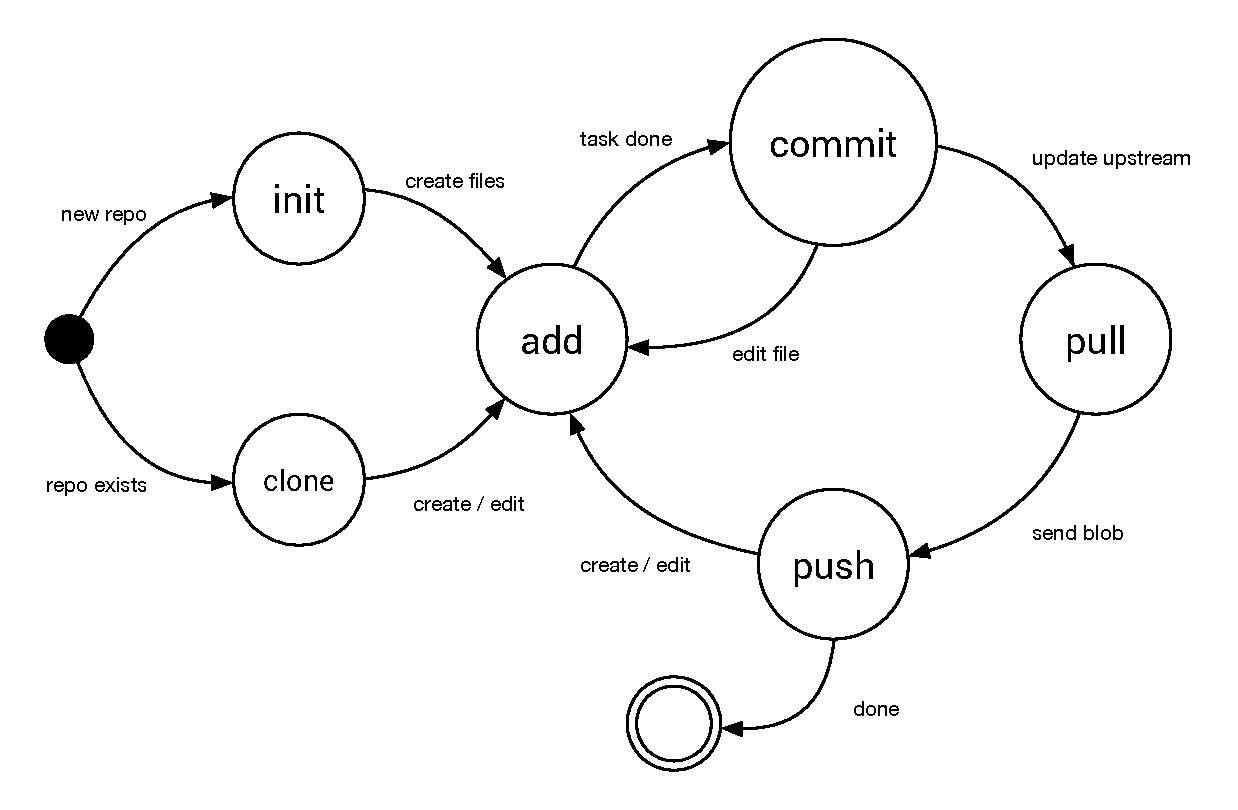
\includegraphics[width=.9\textwidth]{git-command-flow}
        \label{fig:git-command-flow}
    \end{figure}
\end{frame}

\subsection{init}
\begin{frame}{init -{}-bare}
    \Large{\$ git init -{}-bare}
    \begin{figure}
        \center
        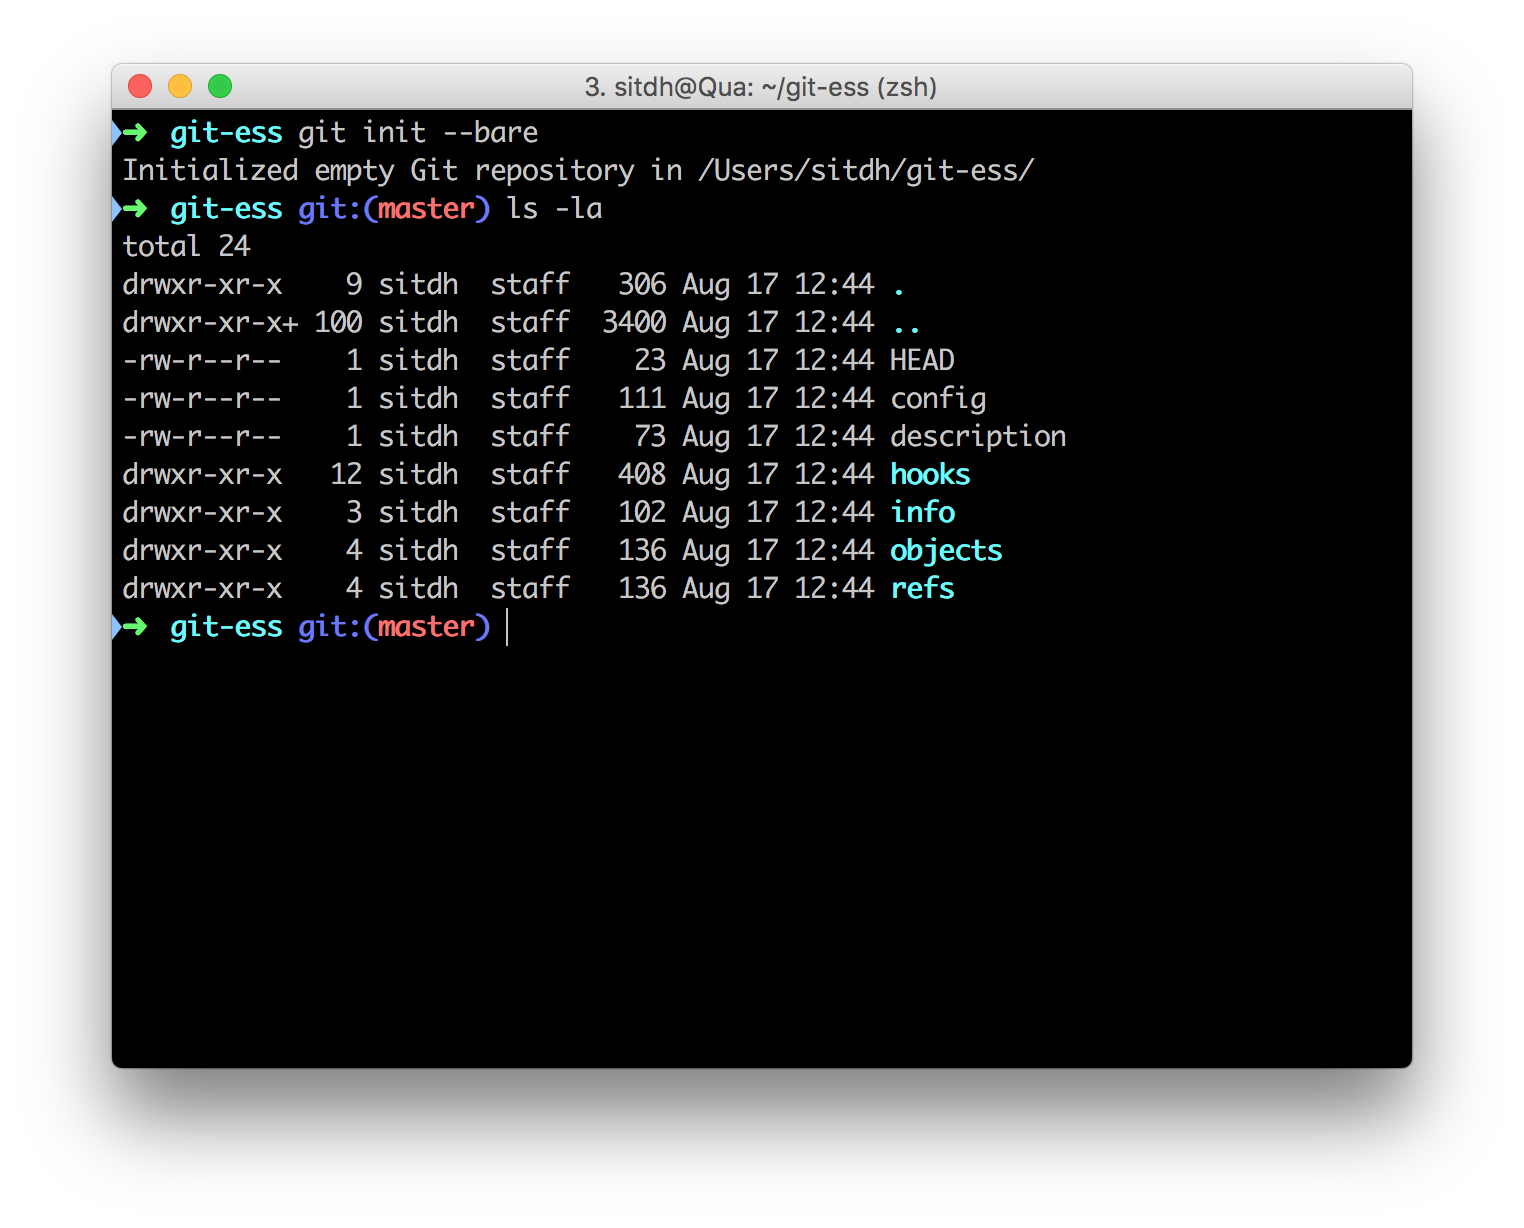
\includegraphics[width=.9\textwidth]{git-init--bare}
        \label{fig:git-init--bare}
    \end{figure}
\end{frame}

\begin{frame}{init}
    \Large{\$ git init}
    \begin{figure}
        \center
        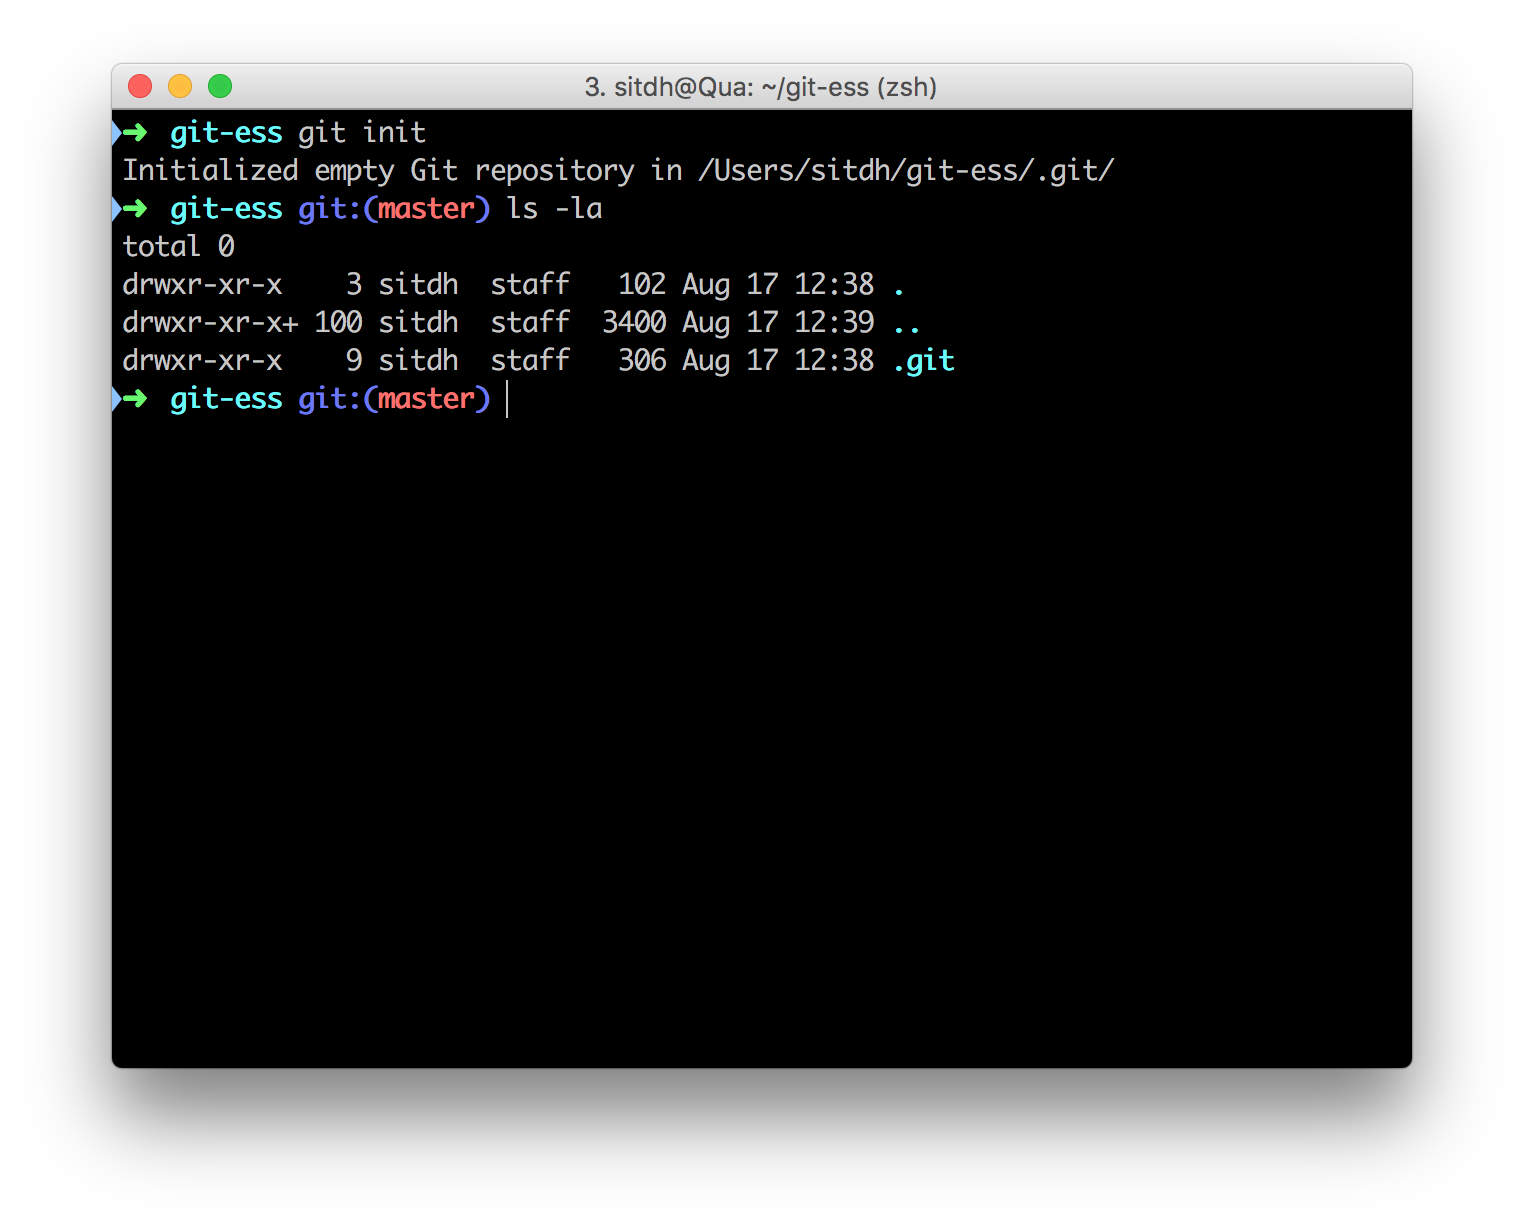
\includegraphics[width=.9\textwidth]{git-init}
        \label{fig:git-init}
    \end{figure}
\end{frame}

\subsection[clone]{clone}
\begin{frame}{Activity flow}
    \begin{figure}
        \center
        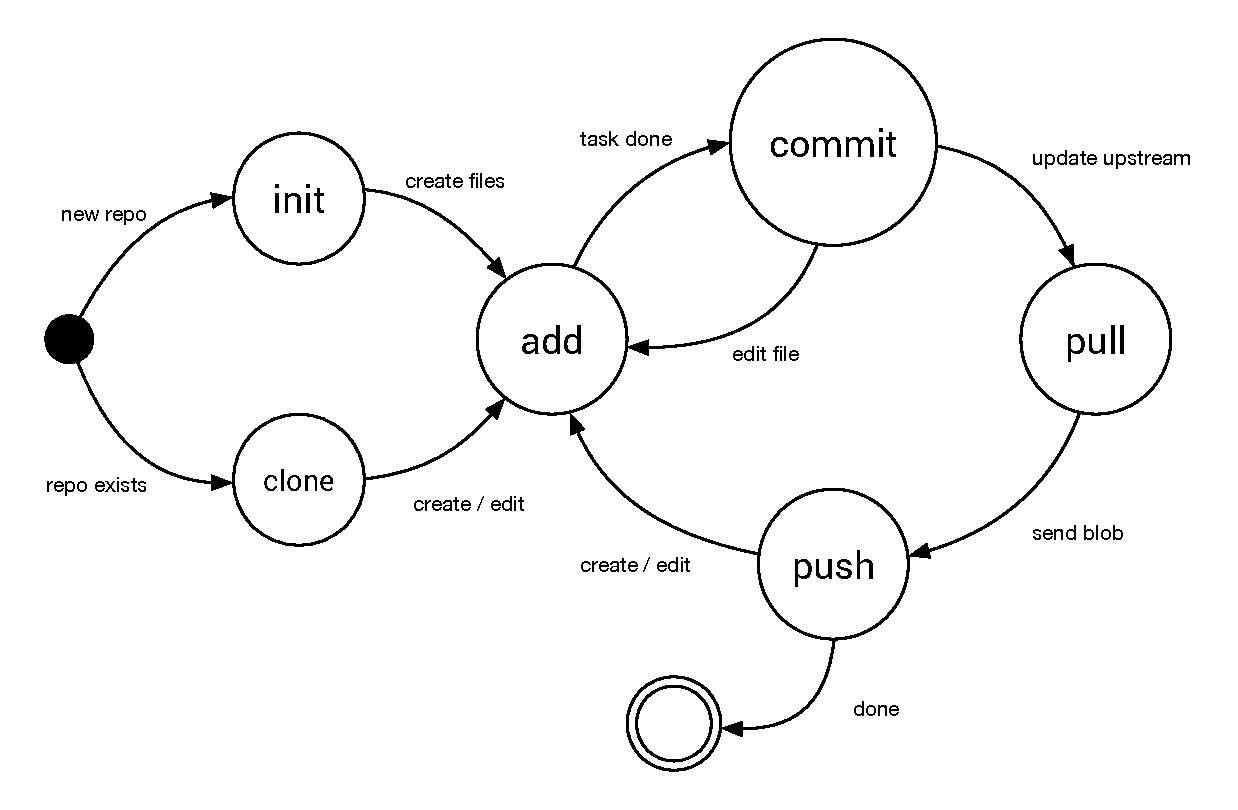
\includegraphics[width=.9\textwidth]{git-command-flow}
        \label{fig:git-command-flow}
    \end{figure}
\end{frame}

\begin{frame}{clone}
    \begin{figure}
        \center
        \includegraphics<1>[width=.7\textwidth]{git-clone-action-0}
        \includegraphics<2>[width=.7\textwidth]{git-clone-action-1}
    \end{figure}
\end{frame}

\begin{frame}{clone}
    \only<1->{
        \textcolor<2->{gray}{\,\,\,\,\Large{\$ git clone \em{"Repo" ["Dest"]}} \newline}
    }
    \only<2->{
        \Large{\$ git clone \textcolor<3>{red}{\,git-ess} \textcolor<4>{red}{\,gitess}}
    }
    \begin{figure}
        \center
        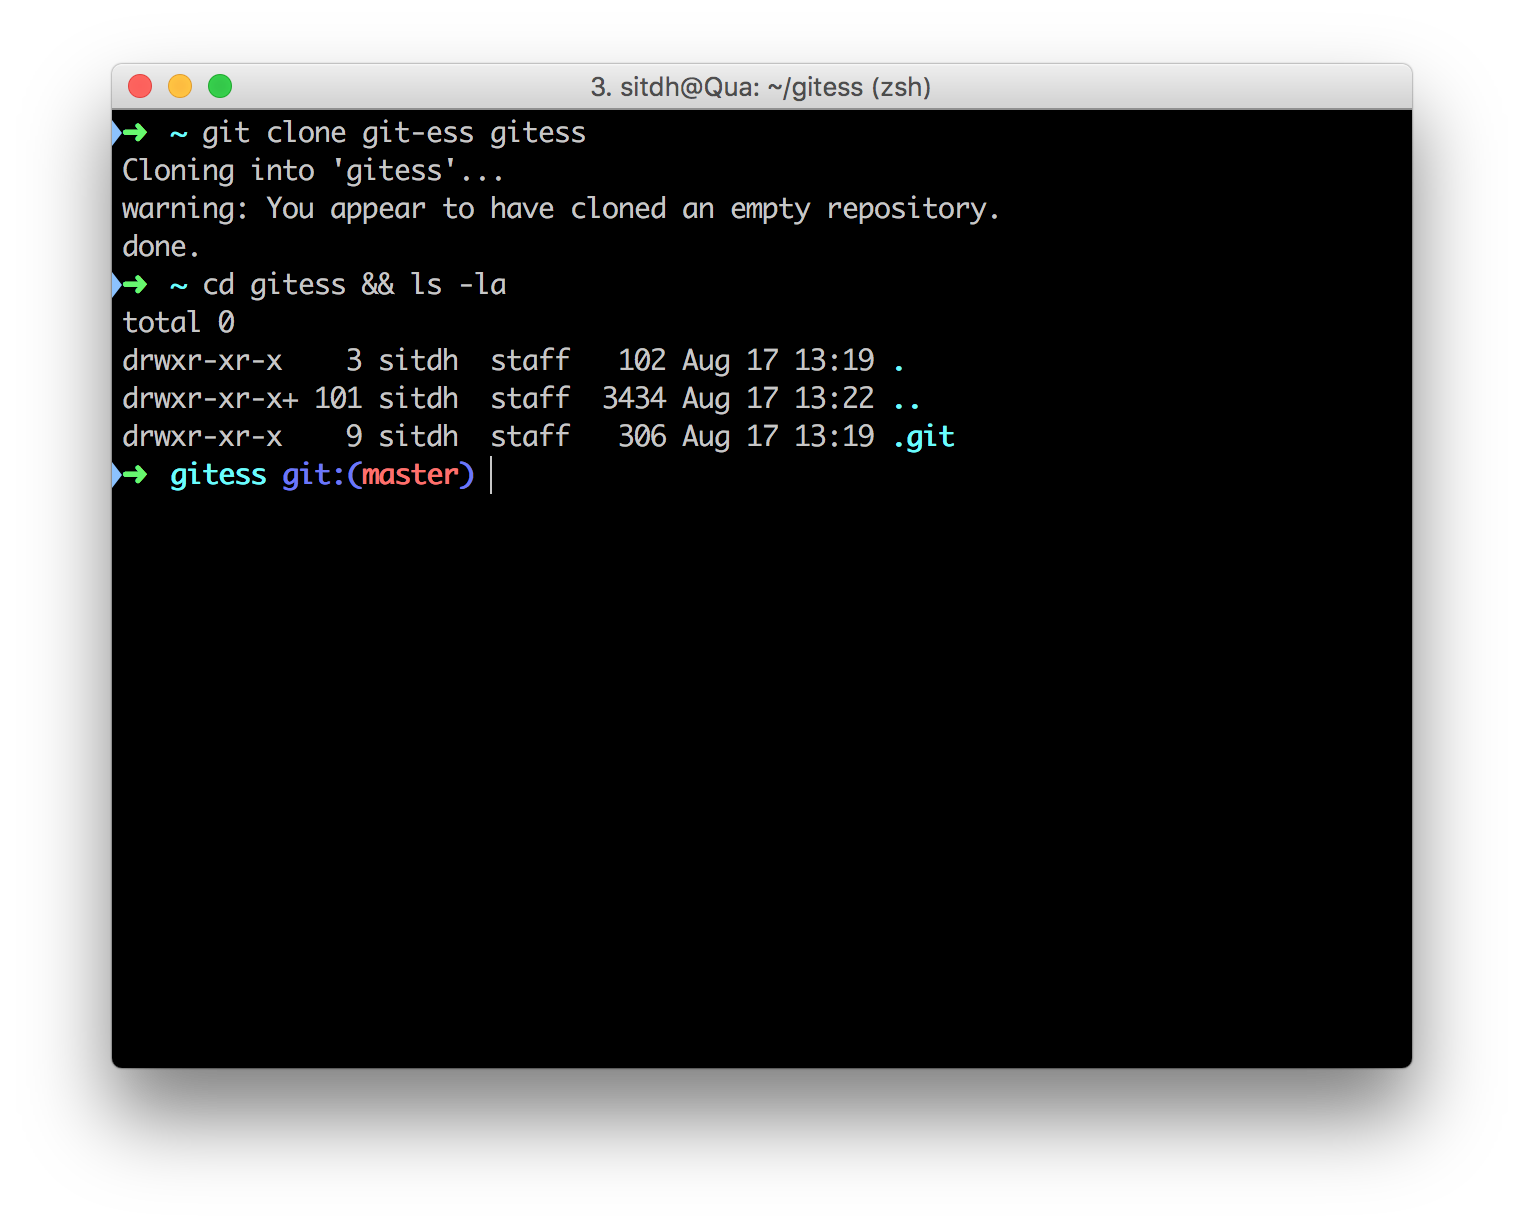
\includegraphics[width=.9\textwidth]{git-clone}
        \label{fig:git-clone}
    \end{figure}
\end{frame}

\begin{frame}{Exercise I: Create and clone \textbf{local repository}}

    \only<1>{
        \textbf{Create local repository}
        \begin{enumerate}[\$]
            \item cd /opt/path
            \item mkdir git-repo \&\& cd "\$\_" 
            \item git init -{}-bare
        \end{enumerate}
    }

    \only<2->{
        \textbf{Clone local repository}
        \begin{enumerate}[\$]
            \item \Large{cd \textasciitilde}
            \item \Large{git clone \textbf<3>{/opt/path/git-repo} \textbf<4>{git\_repo}}
        \end{enumerate}
    }

\end{frame}

\subsection[add]{add}
\begin{frame}{Activity flow}
    \begin{figure}
        \center
        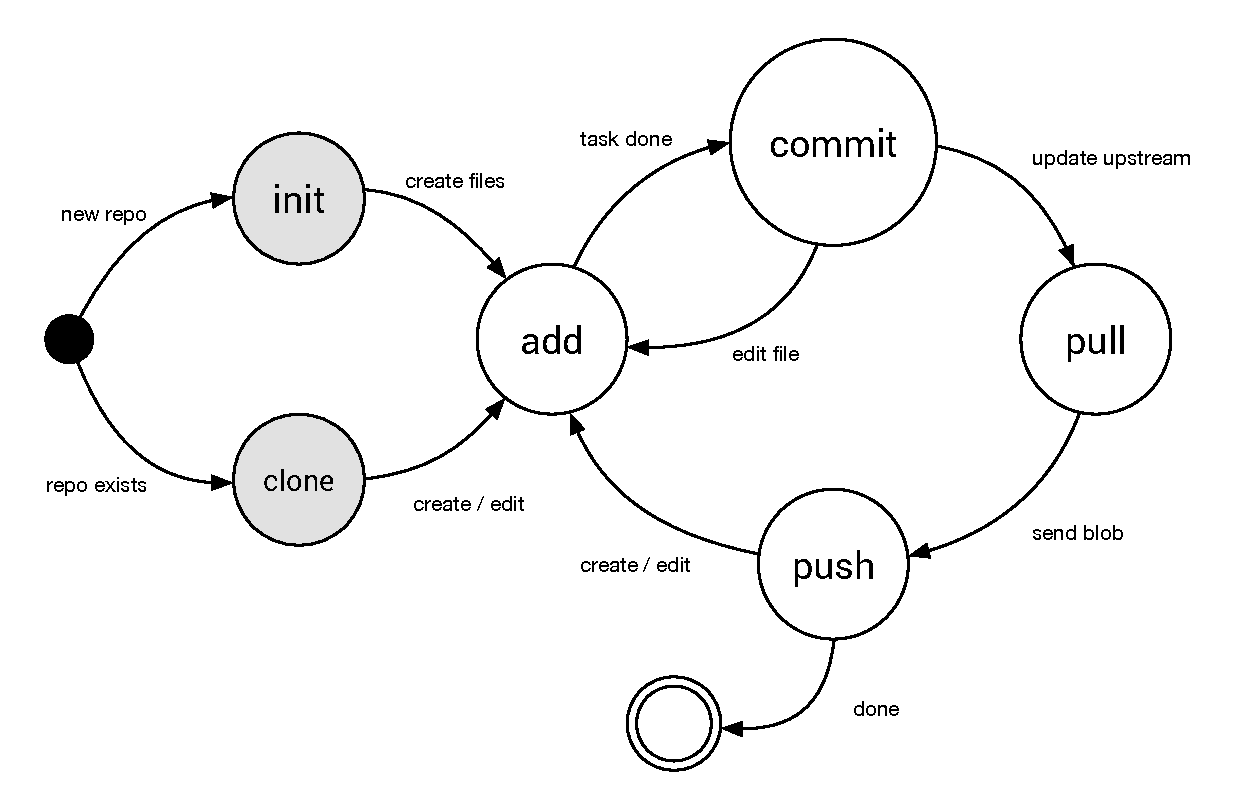
\includegraphics[width=.9\textwidth]{git-command-flow-1}
        \label{fig:git-command-flow-1}
    \end{figure}
\end{frame}

\begin{frame}{unstage \& staged}
    \begin{figure}
        \center
        \includegraphics<1>[width=.8\textwidth]{project-changed-0}
        \includegraphics<2>[width=.8\textwidth]{project-changed-1}
        \includegraphics<3>[width=.8\textwidth]{project-changed-2}
        \includegraphics<4>[width=.8\textwidth]{project-changed-3-2}
        \includegraphics<5>[width=.8\textwidth]{project-changed-3-1}
        \includegraphics<6>[width=.8\textwidth]{project-changed-4}
        \label{fig:project-changed}
    \end{figure}
    \small{https://git-scm.com/book/en/v2/Git-Basics-Recording-Changes-to-the-Repository}
\end{frame}

\begin{frame}{add}
    \begin{enumerate}[\$]
        \item<1-> \textcolor<2>{gray}{\Large{git add \em{/opt/path/get\_repo}}}
        \item<2> \Large{git add .}
    \end{enumerate}
\end{frame}

\begin{frame}{Exercise II: Add files to index}
    \begin{enumerate}[\$]
        \item<1->touch .gitignore {\textbackslash} \newline
            \&\& echo ".DS\_Store{\textcolor{red}{{\textbackslash}n}}bower\_components/" > .gitignore
        \item<3-> touch composer.json
        \item<3-> touch phpunit.xml
        \item<3-> touch phpunit.phar
        \item<4-> git add .
    \end{enumerate}
    
\end{frame}

\subsection[commit]{commit}
\begin{frame}{Activity flow}
    \begin{figure}
        \center
        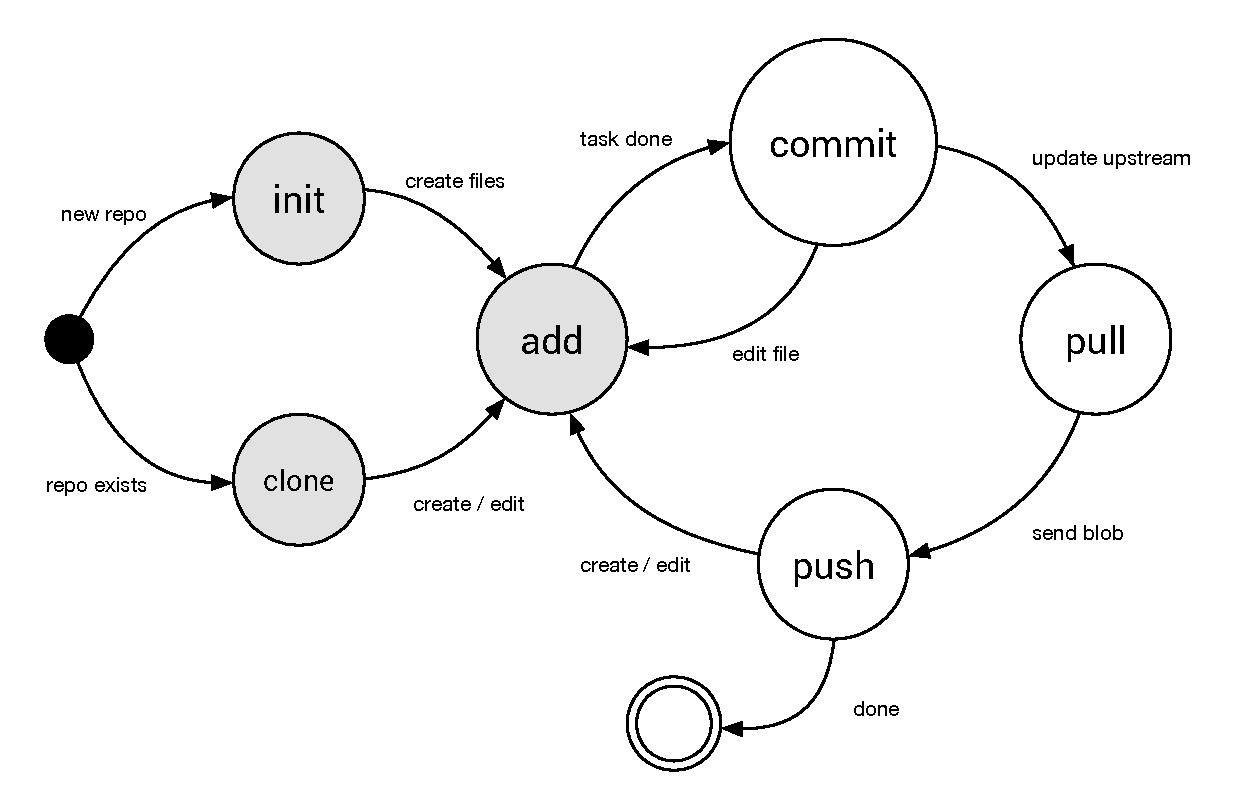
\includegraphics[width=.9\textwidth]{git-command-flow-2}
        \label{fig:git-command-flow-2}
    \end{figure}
\end{frame}

\begin{frame}{commit}
    \begin{figure}
        \center
        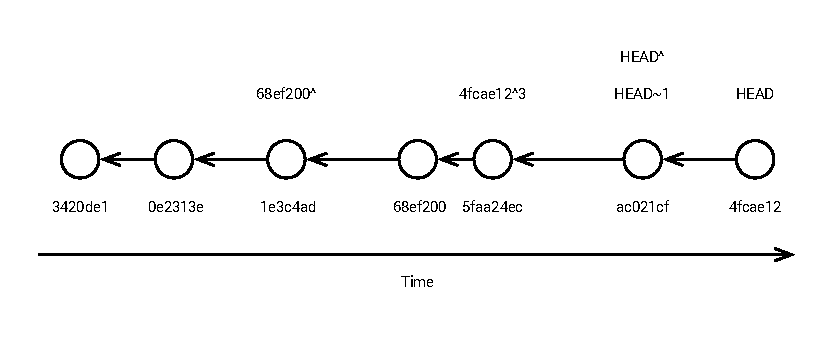
\includegraphics[width=.9\textwidth]{git-commit-flow}
        \label{fig:git-commit-flow}
    \end{figure}
\end{frame}

\begin{frame}{commit}
    \begin{enumerate}[\$]
        \item<1-> \Large{\textcolor<3->{gray}{git commit -am \textcolor<2>{blue}{"Commit message"}}}
        \item<3-> \Large{git commit {\textbackslash}\newline 
            -m \textcolor<4->{blue}{"Update lib version for issue \#32"} {\textbackslash}\newline 
            \textcolor<5->{red}{config.json}}
    \end{enumerate}
\end{frame}

\begin{frame}[t]{commit message}
    \begin{enumerate}
        \item<1-> \textcolor<3->{gray}{Separate subject from body with a blank line}
        \item<3-> \textcolor<6->{gray}{Limit the subject line to 50 characters \newline 
            and wrap the body at 72 characters}
        \item<6-> \textcolor<9->{gray}{Capitalize the subject line}
        \item<9-> \textcolor<10->{gray}{Do not end the subject line with a period}
        \item<10-> \textcolor<13->{gray}{Use the imperative mood in the subject line}
        \item<13-> Use the body to explain \texttt{what} and \texttt{why} vs. \texttt{how}
    \end{enumerate}

    % Heading 
    \only<2>{
        \textbf{Derezz the master control program} \newline

        MCP turned out to be evil and had become intent on world domination.
        This commit throws Tron's disc into MCP (causing its deresolution)
        and turns it back into a chess game.
    }

    % Limit
    \only<4>{
        {\par
        MCP turned out to be evil and had become intent on world domination. This commit throws Tron's disc into MCP (causing its deresolution) and turns it back into a chess game.}
    }

    \only<5>{Derezz the master control program}

    % Capitalize
    \only<7-8>{\textcolor<8>{red}{fix issue \#27} \newline}
    \only<8>{Fix issue \#27}

    % Imperative mood
    \only<11>{\em "Spoken or written as if giving a command or instruction"}
    \only<12>{ 
        \begin{itemize}
            \item Close the door
            \item Take out the trash
            \item Merge branch 'feature'
        \end{itemize}
    }

    % What, Why and How
    \only<14>{
        \begin{itemize}
            \item What side effects does this change have? 
            \item Why is this change necessary?
            \item How does it address the issue?
        \end{itemize}
    }
\end{frame}

\begin{frame}{Exercise III: Commit}
    \begin{enumerate}[\$]
        \item<1-> git commit -m \textbf{'Add ignore list'} .gitignore 
        \item<1-> git commit -m \textbf{'Add composer config'} composer.json
        \item<2-> git commit -am \textbf{'Add testing lib and config'}
            \begin{enumerate}[-]
                \item<3-> \em{phpunit.xml}
                \item<3-> \em{phpunit.phar}
            \end{enumerate}
    \end{enumerate}
\end{frame}

\subsection[pull]{pull}
\begin{frame}{Activity flow}
    \begin{figure}
        \center
        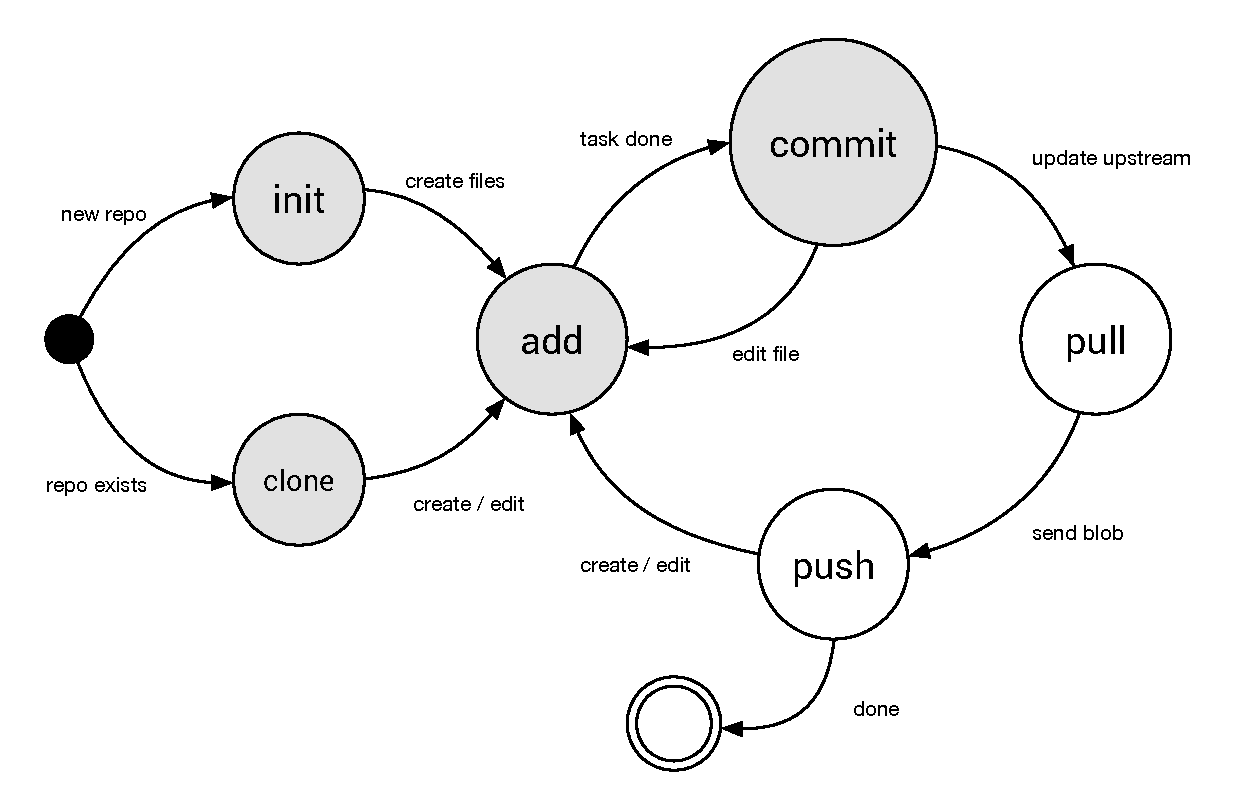
\includegraphics[width=.9\textwidth]{git-command-flow-3}
        \label{fig:git-command-flow-3}
    \end{figure}
\end{frame}

\begin{frame}{pull}
    \Large{
        \[
            Pull = Fetch + Merge
        \]
    }
\end{frame}

\begin{frame}{pull - Sync information}
    \begin{figure}
        \center
        \includegraphics<1>[width=.7\textwidth]{git-pulling-information}
        \label{fig:git-pulling-information}
    \end{figure}
\end{frame}


\begin{frame}{pull - Sync information}
    \begin{figure}
        \center
        \includegraphics<1>[width=.8\textwidth]{git-pull-contents-1}
        \includegraphics<2>[width=.8\textwidth]{git-pull-contents-2}
        \includegraphics<3>[width=.8\textwidth]{git-pull-contents-3}
        \label{fig:git-pull-contents}
    \end{figure}
\end{frame}

\begin{frame}{pull}
    \Large{
        \begin{enumerate}[\$]
            \item<1-> \textcolor<2->{gray}{git pull \em{<remote>} \em{<branch>}}
            \item<2-> git pull \em{origin} \em{master}
        \end{enumerate}
    }
\end{frame}

\subsection{push}
\begin{frame}{Activity flow}
    \begin{figure}
        \center
        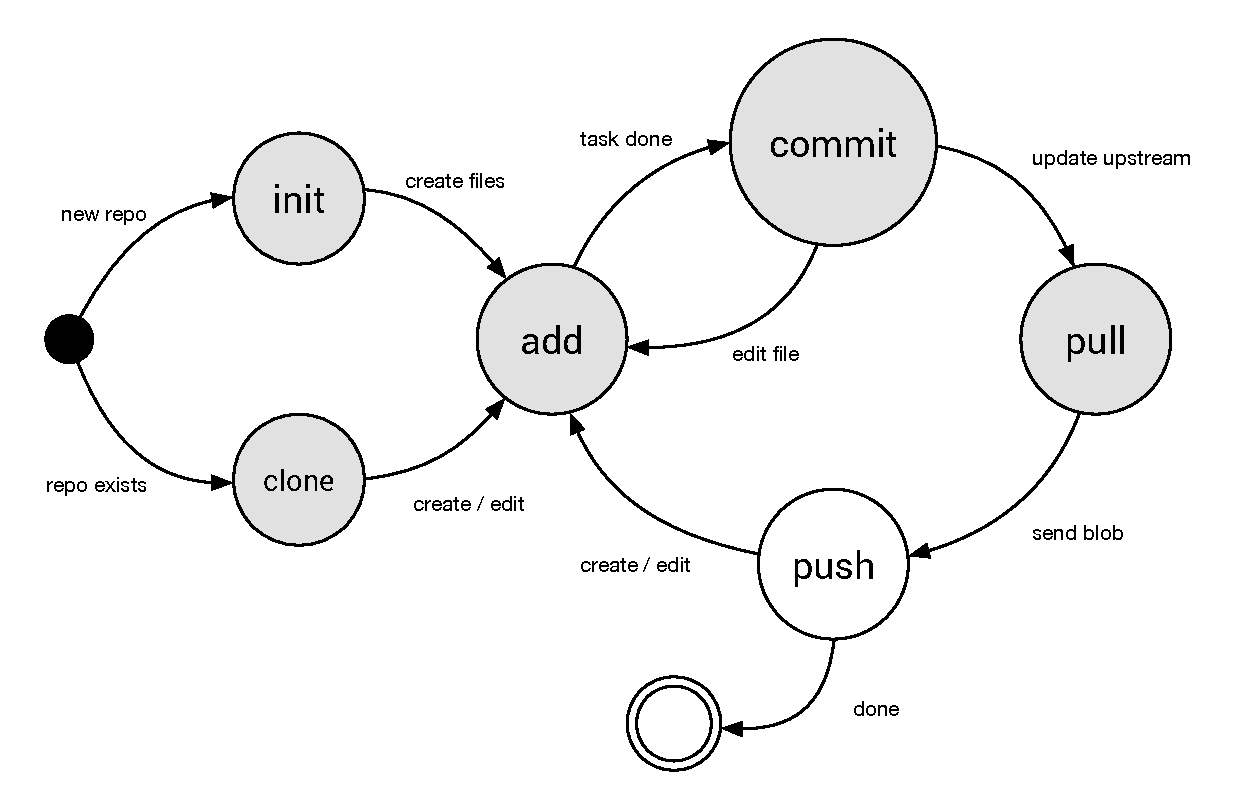
\includegraphics[width=.9\textwidth]{git-command-flow-4}
        \label{fig:git-command-flow-4}
    \end{figure}
\end{frame}

\begin{frame}{push}
    \begin{figure}
        \center
        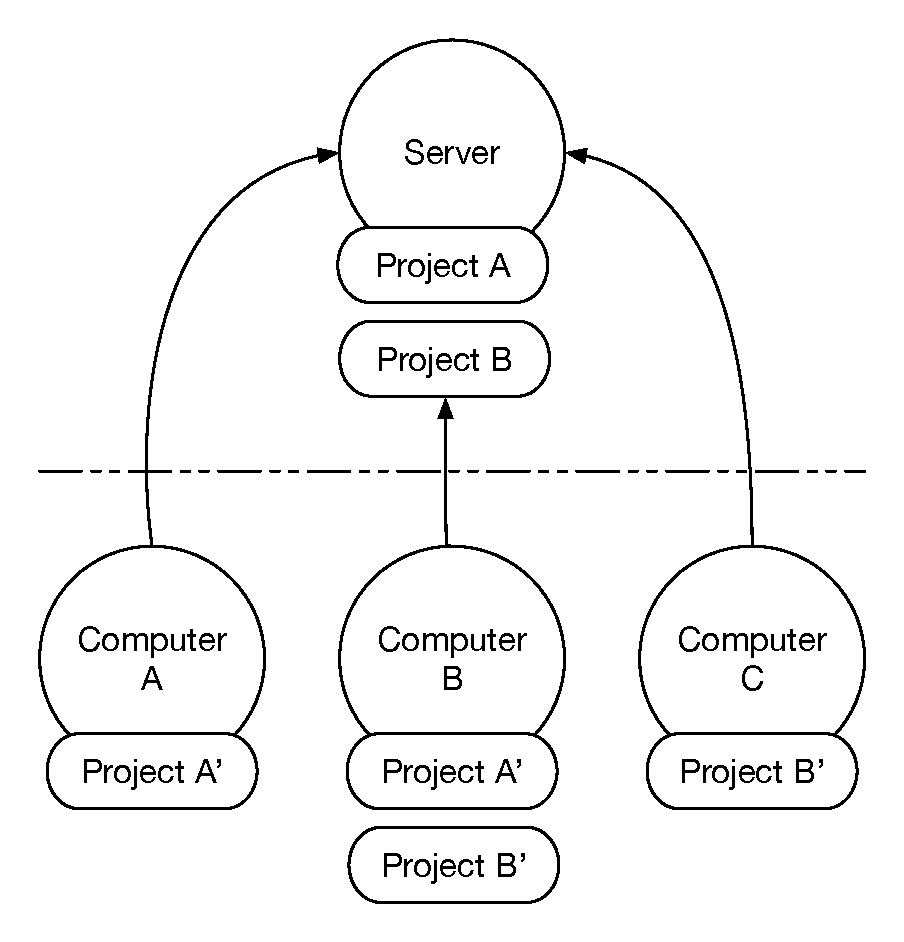
\includegraphics[width=.7\textwidth]{git-push}
        \label{fig:git-push}
    \end{figure}
\end{frame}

\begin{frame}{push}
    \begin{enumerate}[\$]
        \item<1-> \textcolor<2->{gray}{git push \em{<remote>} \em{<branch>} ...}
        \item<2-> git push -u \em{<remote>} \em{<branch>} ...
        \begin{enumerate}[-]
            \item<3-> git push 
        \end{enumerate}
    \end{enumerate}
\end{frame}

\begin{frame}{Exercise IV: Push the source to remote repo}
    \begin{enumerate}[\$]
        \item<1-> \Large{cd {\textasciitilde}/git\_repo}
        \item<2-> \Large{git pull}
        \item<3-> \Large{git push -u origin master}
    \end{enumerate}
\end{frame}

\section{More action}

\begin{frame}{branch}
    \begin{figure}
        \center
        \includegraphics<1>[width=.8\textwidth]{git-branching-0}
        \includegraphics<2>[width=.8\textwidth]{git-branching-1}
        \includegraphics<3>[width=.8\textwidth]{git-branching-2}
        \label{fig:git-branching}
    \end{figure}
\end{frame}

\begin{frame}{branch}
    \begin{enumerate}[\$]
        \item<1-> \textcolor<2->{gray}{
                \Large{git checkout \textbf{<-b> <branch\_name> <start\_point>}}}
        \item<2-> \textcolor<4->{gray}{
                \Large{git checkout \textbf<3->{-b feature}}}
        \item<4-> \textcolor<6->{gray}{
                \Large{git checkout \textbf<4>{-b hotfix} \textbf<5>{1e344ad}}}
        \item<6-> \Large{git checkout \textbf<6->{hotfix ac021cf}}
    \end{enumerate}
\end{frame}

\begin{frame}{merge}
    \begin{figure}
        \center
        \includegraphics<1>[width=.8\textwidth]{git-branching-2}
        \includegraphics<2>[width=.8\textwidth]{git-branching-3}
        \includegraphics<3>[width=.8\textwidth]{git-branching-4}
        \label{fig:git-merging}
    \end{figure}
\end{frame}

\begin{frame}{merge}

    \begin{enumerate}[\$]
        \item<1-> \textcolor<2->{gray}{
                \Large{git merge \textbf{<option> <branch\_name> <commit>}}}
        \item<2-> \textcolor<3->{gray}{
                \Large{git merge \textbf<2->{development}}}
        \item<3-> \Large{git merge \textbf<3->{development 1102efd}}
    \end{enumerate}

    \begin{figure}
        \center
        \includegraphics<1>[width=.8\textwidth]{git-branching-5}
        \includegraphics<2->[width=.8\textwidth]{git-branching-6}
        \label{fig:git-current-branch}
    \end{figure}
\end{frame}

\begin{frame}{Recommended branches}
    \begin{figure}
        \center
        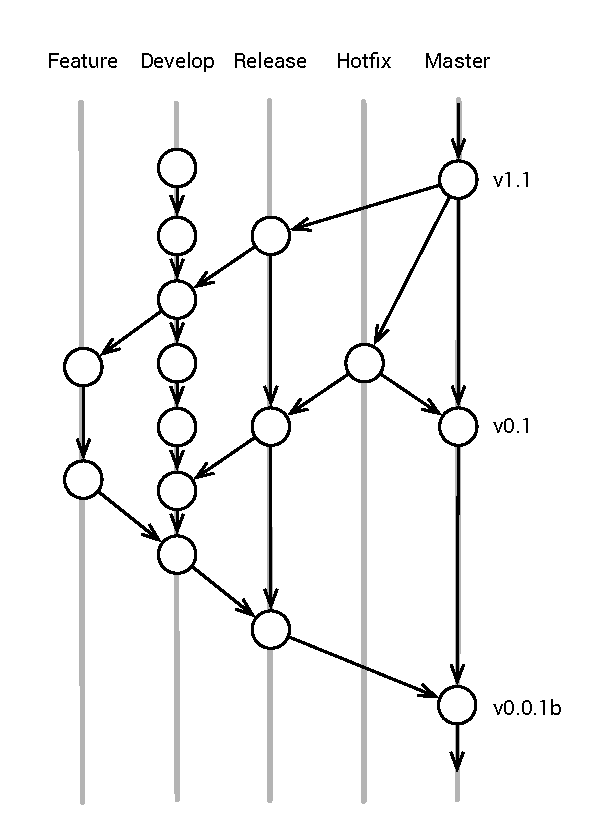
\includegraphics[height=.8\textheight]{git-recommended-branches}
        \label{fig:git-recommanded-branches}
    \end{figure}
\end{frame}

\section{Best practise}
\begin{frame}{Best practise}
    \begin{figure}
        \center
        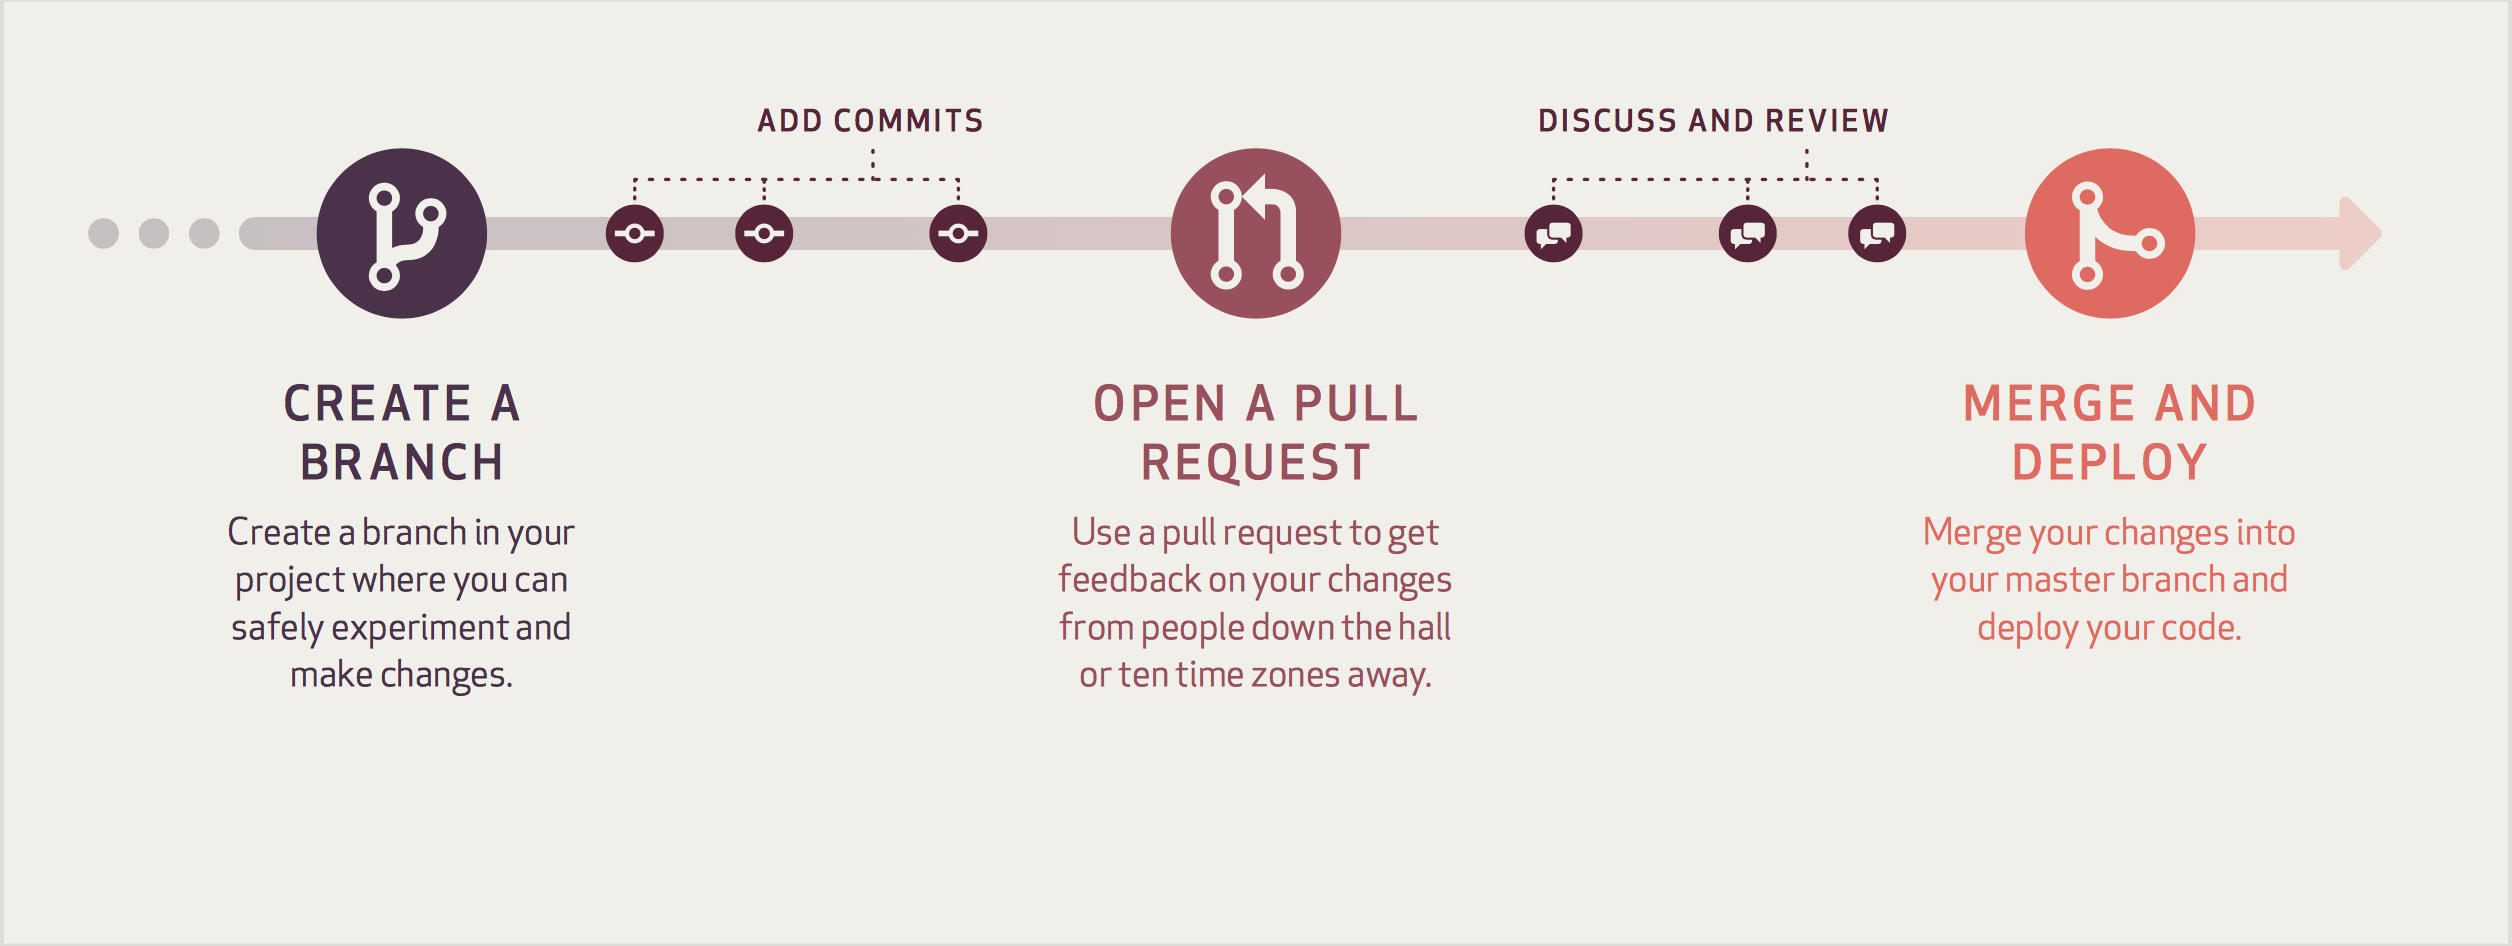
\includegraphics[width=.9\textwidth]{git-workflow}
        \caption{https://guides.github.com/introduction/flow/}
        \label{fig:git-workflow}
    \end{figure}
\end{frame}

\begin{frame}{git-flow}
    \begin{figure}
        \center
        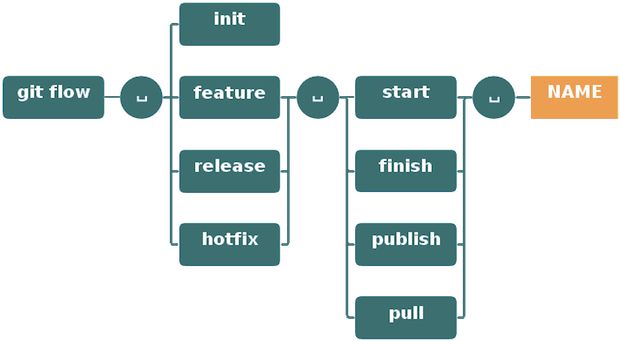
\includegraphics[width=.9\textwidth]{git-flow-commands}
        \label{fig:git-flow-commands}
    \end{figure}
    \center{https://danielkummer.github.io/git-flow-cheatsheet/}
\end{frame}

\section{Workshop}
\begin{frame}{GitHub - Happy coding}
    \begin{itemize}
        \item Create Remote repository on GitHub
        \item Sync remote source
        \item Collaboration overview
    \end{itemize}
\end{frame}

\begin{frame}{Exercise V: Create remote repository on GitHub}
    \only<1>{
        \begin{figure}
            \center
            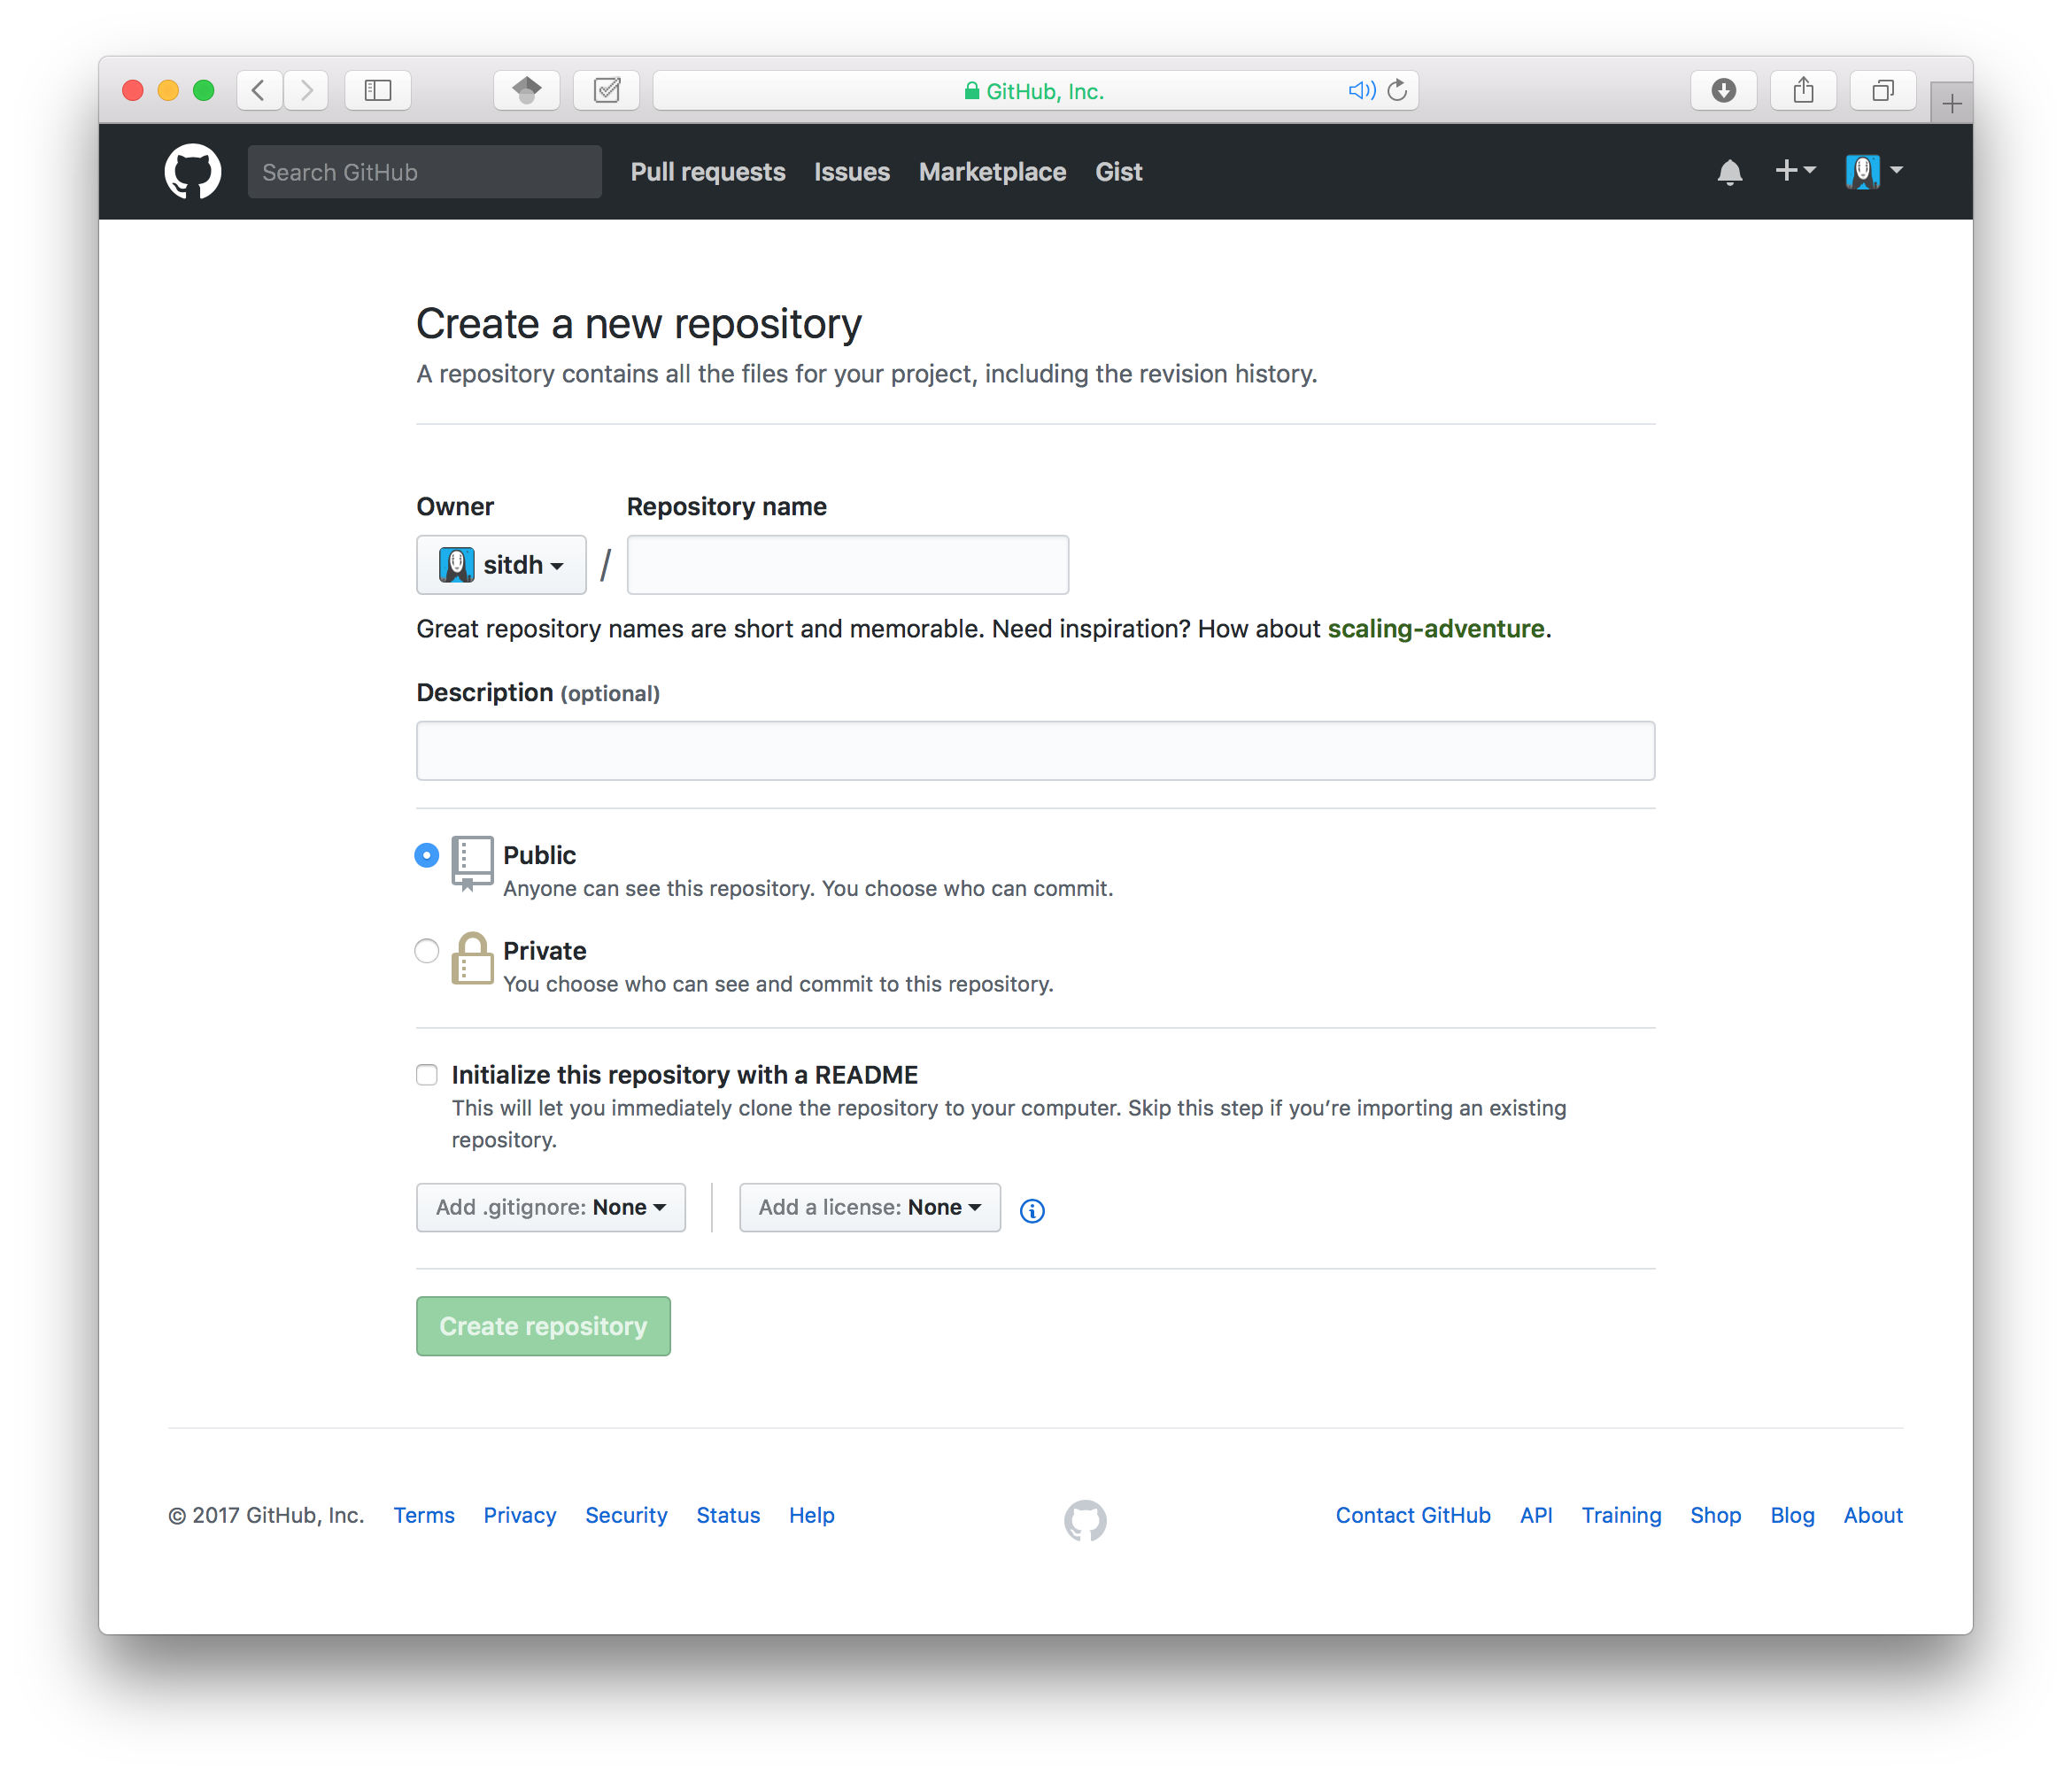
\includegraphics[width=.8\textwidth]{create-a-new-repository}
            \label{fig:create-a-new-repository}
        \end{figure}
    }

    \only<2>{
        \begin{figure}
            \center
            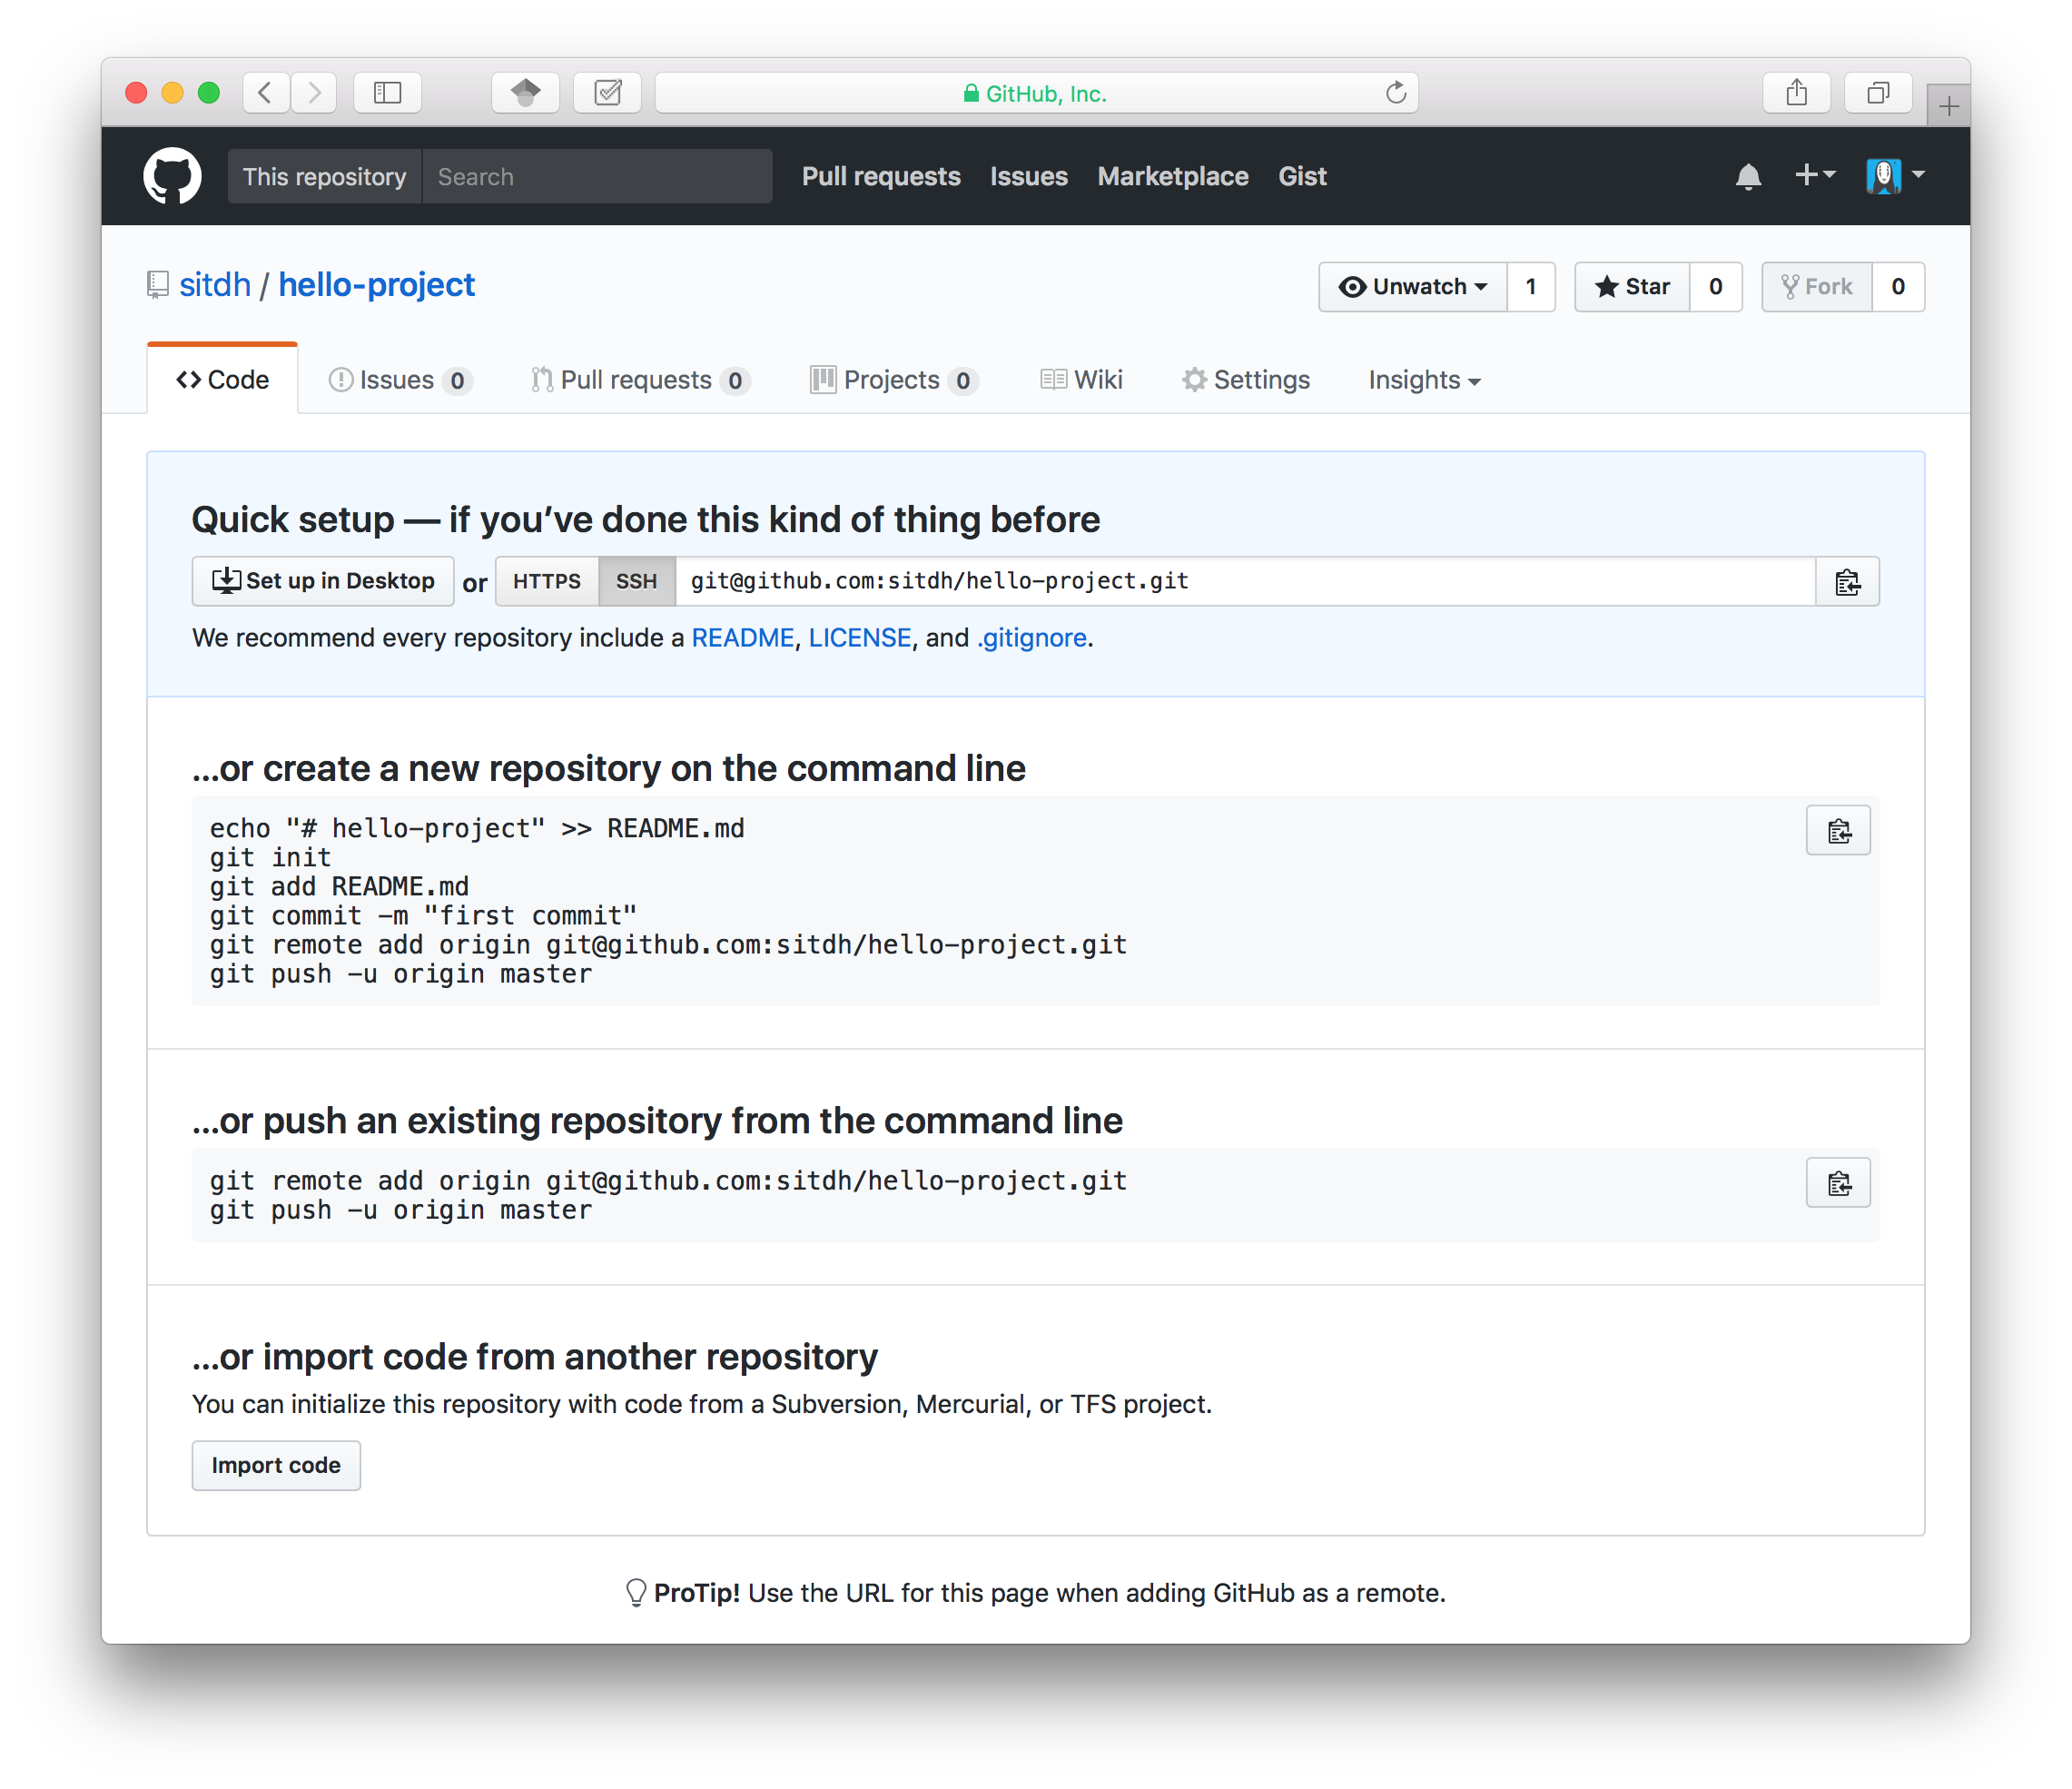
\includegraphics[width=.8\textwidth]{create-a-new-repository-1}
            \label{fig:create-a-new-repository-1}
        \end{figure}
    }

    \only<3>{
        \begin{figure}
            \center
            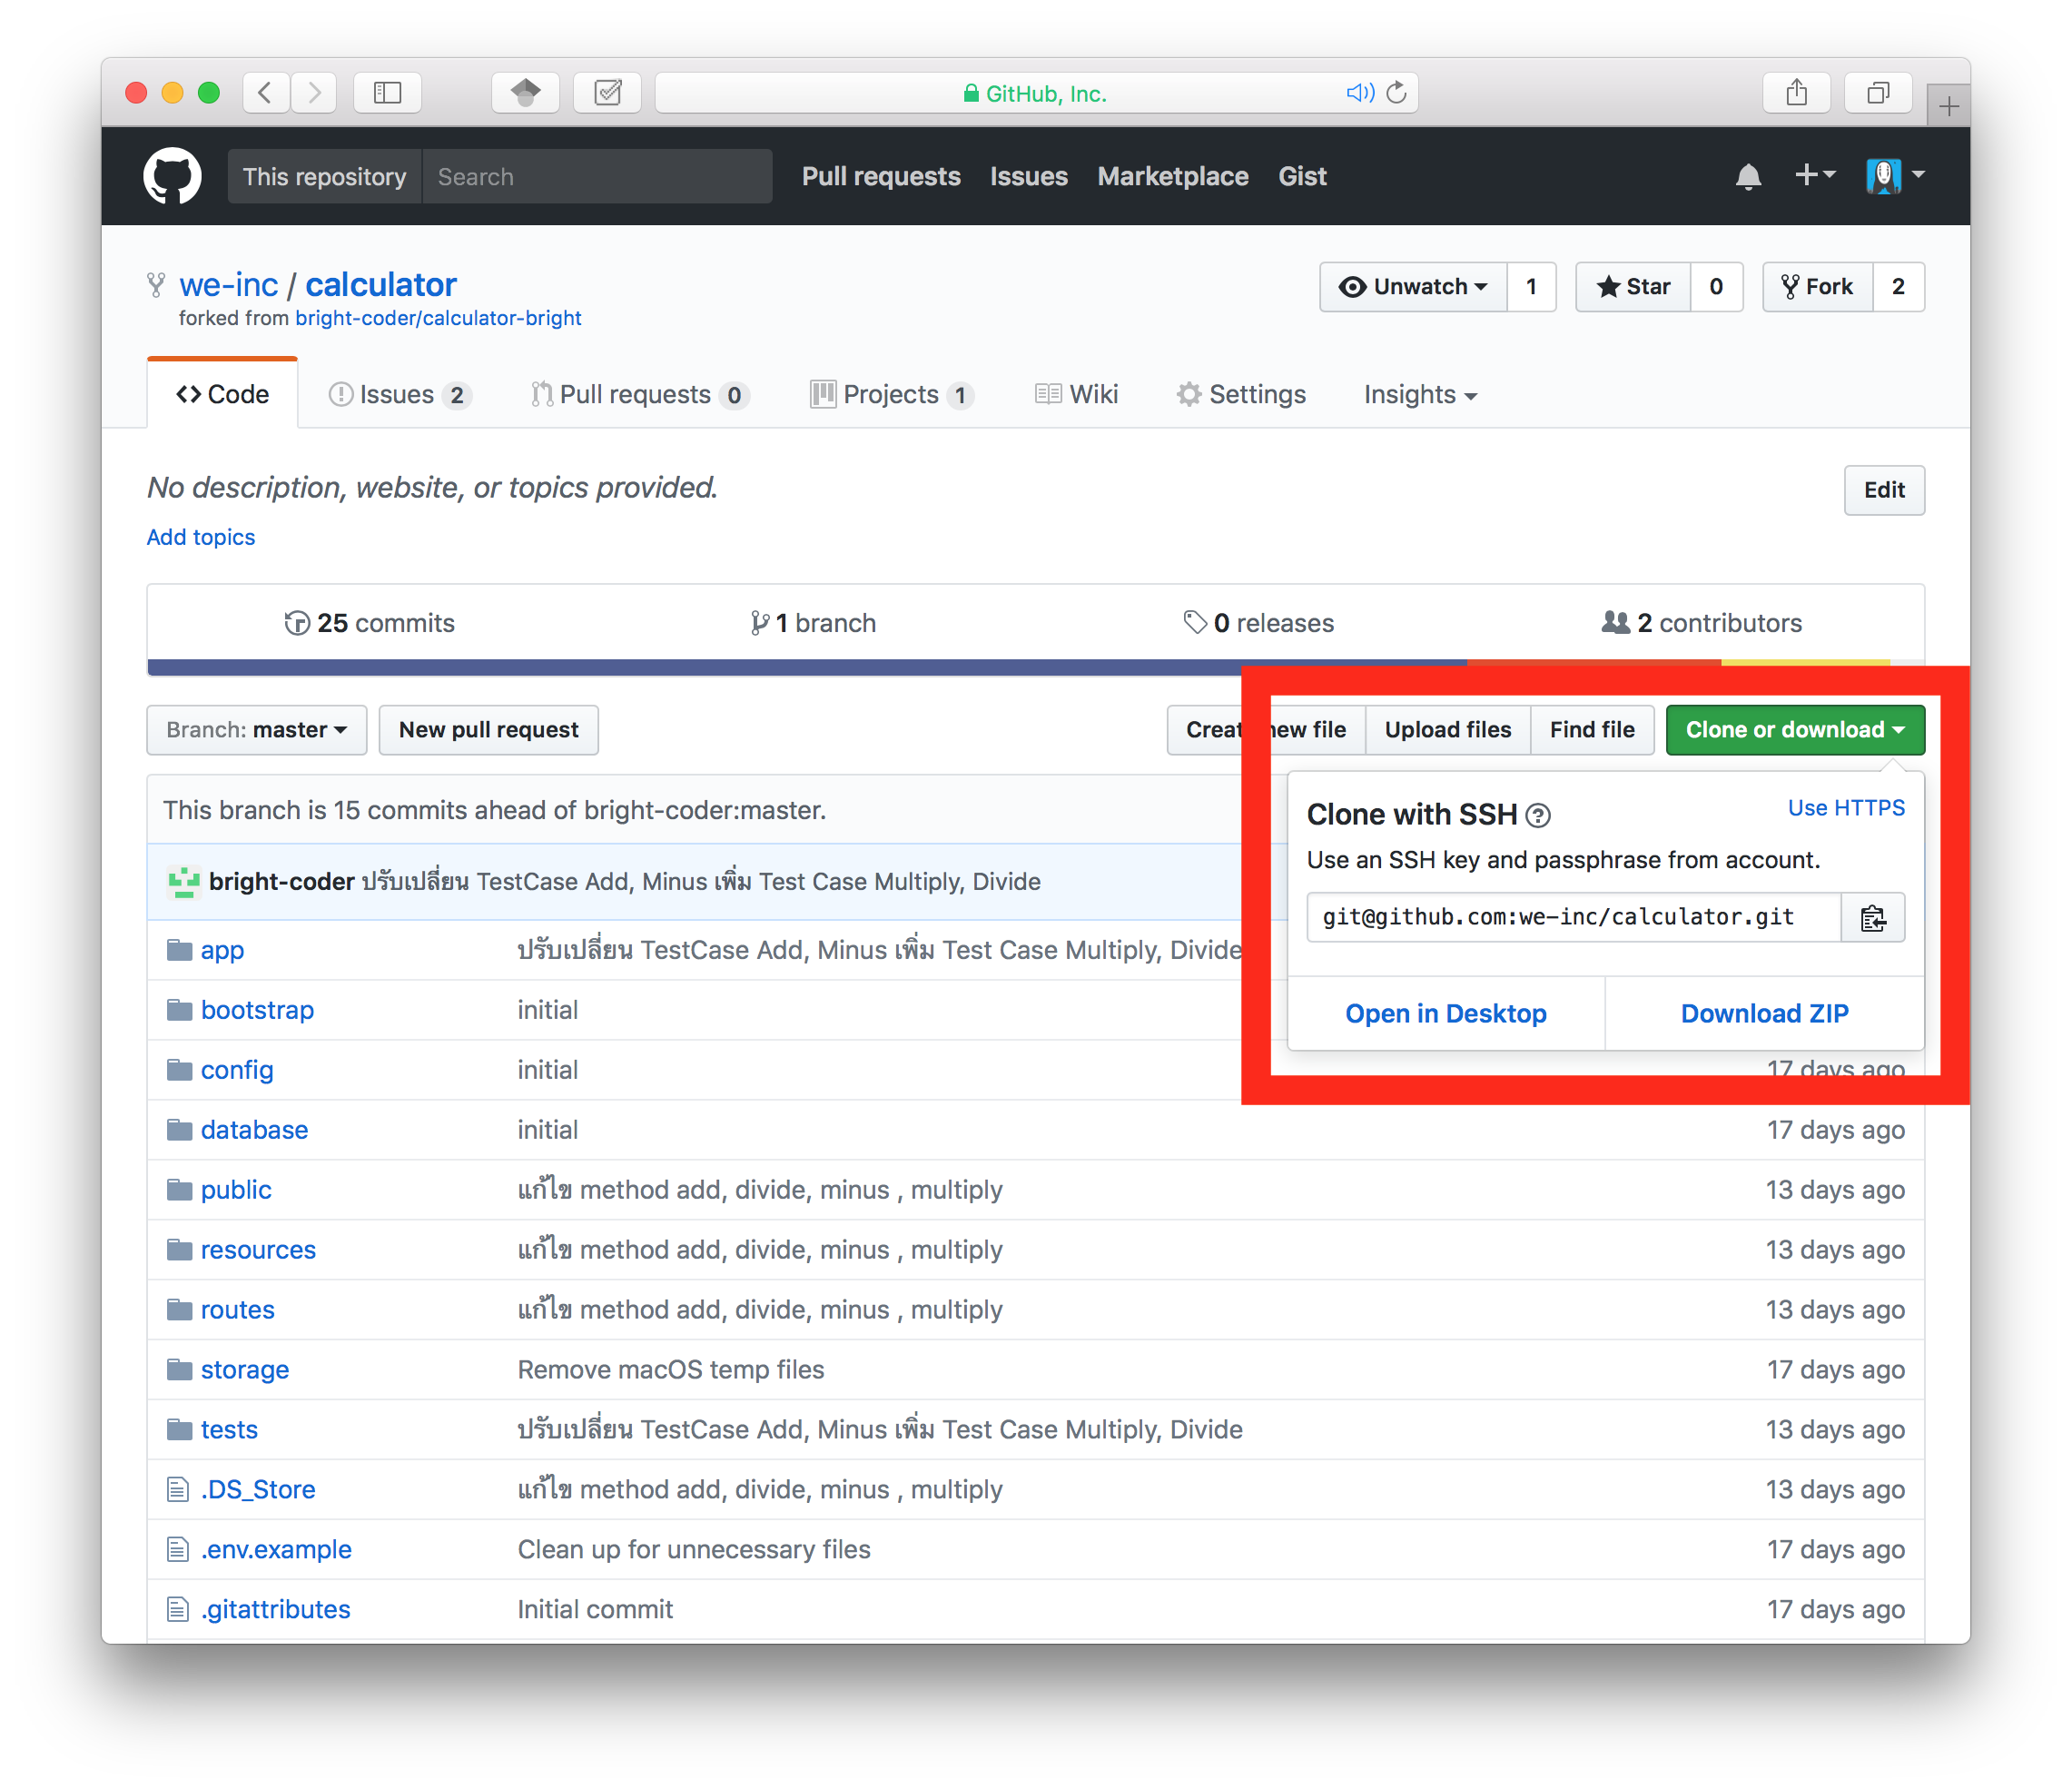
\includegraphics[width=.8\textwidth]{git-get-clone-uri}
            \label{fig:git-get-clone-uri}
        \end{figure}
    }
\end{frame}

\begin{frame}{Repository URL}
    \begin{itemize}
        \item<1-> \Large{git@github.com:we-inc/calculator.git}
        \item<1-> \Large{https://github.com/we-inc/calculator.git}
        \begin{itemize}
            \item<2-> \Large{\textbf{Username}, \textbf{Password} are both required}
        \end{itemize}
    \end{itemize}
\end{frame}

\begin{frame}{Add remote repository}
    \begin{enumerate}[\$]
        \item \Large{cd {\textasciitilde}/git\_repo}
        \item \Large{git remote add origin git@github.com:sitdh/hello-project.git}
        \item \Large{git push -u origin master}
    \end{enumerate}
\end{frame}

\begin{frame}{Error}
    \begin{figure}
        \center
        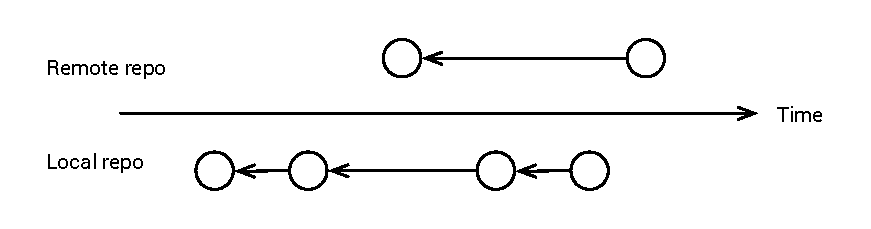
\includegraphics[width=\textwidth]{git-unrelated-histories}
        \label{fig:git-unrelated-histories}
    \end{figure}
\end{frame}

\begin{frame}{Collaboration overview}
\end{frame}

\section{Summary}
\begin{frame}{Summary}
    \texttt{get add \em{<somefile>}} \newline
    \texttt{git pull} \newline
    \texttt{git commit -m \em{"<Some awesome commit message>"}} \newline
    \texttt{git push}
\end{frame}

\section{References}
\begin{frame}{Books}
    \begin{figure}
        
\includegraphics[height=.6\textheight]{progit}
        \label{fig:book-progit}
    \end{figure}
    \center{Pro Git - \small{https://git-scm.com/book/en/v2}}
\end{frame}

\begin{frame}{More info.}
\end{frame}

\begin{frame}
    \begin{figure}
        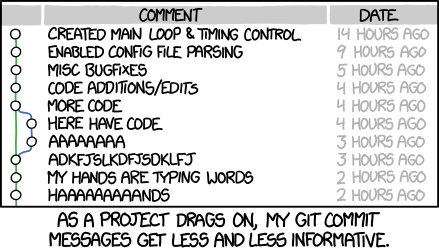
\includegraphics[height=.4\textheight]{git_commit}
        \label{fig:xkcd-git-commit}
    \end{figure}
\end{frame}

\end{document}
